\listfiles
\documentclass{scrartcl}
\usepackage[T1]{fontenc}
\usepackage[ngerman]{babel}
\usepackage{exsheets}
\usepackage{array}
\usepackage{graphicx}
\usepackage{float}
\usepackage[backend=biber,sortcites,defernumbers]{biblatex}
\addbibresource{solution.bib}

\begin{document}

\SetupExSheets{
  question/type = exam ,
  headings = klausur,
  solution/print = true,
  counter-within=section
}

\let\oldsolution\solution

\renewenvironment{solution}{%
	\SetupExSheets{counter-format=}
    \oldsolution
}

\begin{titlepage}
  \centering
  \Huge Theoriepr"ufung DSV-Skilehrer \par
  \vspace{3cm}
  \normalsize
    Diese L"osung wurde nicht von mir selbst erstellt. Ich habe diese L"osung aus mehreren anderen L"osungen zus"atzlich einiger Erg"anzungen zusammengestellt. Anmerkungen oder Fragen k"onnen gerne an mich gestellt werden.\\
  Es gibt einige Fragen mit Kursiv geschriebenen Abchnitten und / Trennzeichen. Dies ist als Auswahl zu verstehen, und in der tats"achlichen Frage steht nur eine der M"oglichkeiten.\\
\end{titlepage}

\tableofcontents
\section{Sportorganisation}

\begin{question}{1}
Mit welcher Qualifikation ist man berechtigt, eine DSV-Skischule zu f"uhren? Nennen sie alle Qualifikationsm"oglichkeiten.
\end{question}
\begin{solution}
\begin{itemize}
\item DSV-Skilehrer
\item Instructor mit Skischulleiter Ausbildung
\end{itemize}
Quelle nicht gefunden.
\end{solution}

\begin{question}{2}
Welche Voraussetzungen m"ussen erf"ullt sein, um als Skischule den Status DSV-Skischule zu erhalten?
\end{question}
\begin{solution}
\begin{itemize}
\item Erf"ullung des Kriterienkatalogs des DSV und der Landesskiverb"ande
\item Regelm"a"sige Fortbildung der Skischulleiter alle 2 Jahre
\end{itemize}
\citetitle{theorie} Seite 93
\end{solution}

\begin{question}{5}
Geben Sie einen "Uberblick zur IVSI. Gehen Sie dabei auf die Bedeutung f"ur die Ausbildung im DSV ein.
\end{question}
\begin{solution}
\begin{itemize}
\item IVSI = Internationaler Verband der Schneesport-Instruktoren
\item Zusammenschluss nicht professioneller, aber ausgebildeter und gepr"ufter Lehrkr"afte in den Disziplinen Ski-Alpin, Snowboard, Skitour, Telemark und Nordic.
\item Die Ausbildungsgrundlage stellen die Mindestanforderungen f"ur die Ausbildung in den Mitgliedsverb"anden.
\item Die IVSI-Marke ist eine international einheitliche Marke f"ur den Instruktoren-Ausweis und dient als Nachweis f"ur eine qualifizierte Aus- und Fortbildung. Auch der DSV vergibt die IVSI-Marke.
\end{itemize}
\citetitle{theorie} Seite 53
\end{solution}

\begin{question}{4}
Skizzieren Sie die nationale und internationale Struktur des Schneesports.
\end{question}
\begin{solution}

  \begin{table}[H]
    \label{strukturschneesport}
    \scriptsize
    \begin{center}
    \begin{tabular}{p{2,5cm}|p{5,5cm}|p{5,5cm}}
        & \textbf{Fachlich} & \textbf{"Uberfachlich}\\
    \hline
      International & Interski International (IVSS, IVSI, ISIA), IBU, FIS & IOC\\
      National (Bund) & Interski Deutschland (DVS) & DOSB, DSH
    \end{tabular}
    \end{center}
  \end{table}

  \citetitle{theorie} Seite 44

\end{solution}

\begin{question}{4}
Welche Ausbildungsm"oglichkeiten bietet der DSV seinen Mitgliedern im Leistungs- und Breitensport?
\end{question}
\begin{solution}

  \begin{table}[H]
    \label{ausbildungen}
    \scriptsize
    \begin{center}
      \begin{tabular}{p{6,75cm}|p{6,75cm}}
        \textbf{Leistungssport} & \textbf{Breitensport}\\
      \hline
        Trainer A, B, C, Sportwissenschaftler (in Kooperation mit der Uni Leipzig), Mit Trainer A Diplomtrainer m"oglich, IHK Wirtschafts-/Sportfachwirt & Trainer A, B, C, Skischulleiter, IHK Wirtschafts-/Sportfachwirt
      \end{tabular}
    \end{center}
  \end{table}

  \citetitle{theorie} Seite 66-67

\end{solution}

\begin{question}{5}
Geben Sie einen "Uberblick zu INTERSKI DEUTSCHLAND (DVS) und nennen Sie f"unf Mitgliedsverb"ande.
\end{question}
\begin{solution}
Dachverband derjenigen  Mitgliedsverb"ande, die sich mit Unterricht und Ausbildung im Schneesport befassen. Dazu z"ahlen: Berufsverb"ande, Amateurverb"ande sowie sonstige Verb"ande, Organisationen und Beh"orden, zu deren Aufgaben die Aus-, Weter- und Fortbildung im Schneesport geh"oren. Mitglieder sind:
\begin{itemize}
\item Deutscher Skiverband (DSV)
\item Deutscher Skilehrerverband (DSLV)
\item Deutscher Alpenverein (DAV)
\item Deutscher Turnerbund (DTB)
\item Naturfreunde Deutschlands
\item Arbeitsgemeinschaft Schneesport an Hochschulen (ASH)
\item Bundesministerium f"ur Verteidigung f"ur den Bereich der Bundeswehr
\item Bayrisches Polizeisportkuratorium
\item Deutscher Behindertensportverbad (DBS)
\end{itemize}
\citetitle{theorie} Seite 68-70
\end{solution}

\begin{question}{3}
Beschreiben Sie die Struktur des Deutschen Skiverbandes e.V. und der DSV Gesellschaften.
\end{question}
\begin{solution}
Der DSV ist die Muttergesellschaft dreier unter seinem Dach gegr"undeter GmbHs. Der DSV e.V. gew"ahrleistet den gemeinn"utzigen Teil der gesamten Vereinsarbeit. Alle wirtschaftlichen und vermarktungsrelevanten Aktivit"aten sind ausgegliedert und den drei Gesellschaften Leistungssport, Marketing und Verwaltung zugeordnet.\\
Die drei GmbHs sind durch Lizenz-, Leistungs- und Mietvertr"age mit dem DSV als Muttergesellschaft eng verbunden. Sie sind untereinander durch Agentur- und Leistungsvertr"age verkn"upft und werden jeweils von Aufsichtsr"aten und Gesch"aftsf"uhrern geleitet und verwaltet. Der DSV-Pr"asident hat jeweils den Vorsitz in den Aufsichtsr"aten der Leistungssport und Marketing GmbH. Der DSV-Schatzmeister ist in allen drei Aufsichtsr"aten t"atig und zugleich Aufsichtsratsvorsitzender der Verwaltungs GmbH.\\\\
\citetitle{theorie} Seite 75
\end{solution}

\begin{question}{5}
Was ist das oberste Verbandsorgan im DSV? Beschreiben Sie dessen Mitglieder und Aufgaben.
\end{question}
\begin{solution}
Oberstes Verbandsorgan: Verbandsversammlung\\
Mitglieder:
\begin{itemize}
\item Ordentliche und au"serordentliche Mitglieder des DSV
\item Pr"asidium
\item Vorsitzende der Ausch"usse und Referate
\item Fachreferenten
\item Gesch"aftsf"uhrer der drei GmbHs
\item DSV-Direktoren
\item Sportliche Leiter
\end{itemize}
Aufgaben:
\begin{itemize}
\item Entgegennahme der Berichte des Pr"asidiums
\item Genehmigung des Stellenplans f"u Ehren- und Hauptamt
\item "Anderung und Beschluss aller Ordnungen und der Satzung
\end{itemize}
\citetitle{theorie} Seite 80-81
\end{solution}

\begin{question}{5}
Was ist das oberste Gremium des Bereichs DSV-Sportentwicklung? Beschreiben Sie dessen Mitglieder und Aufgaben.
\end{question}
\begin{solution}
Oberstes Gremium: Jahreskonferenz Sportentwicklung\\
Mitglieder:
\begin{itemize}
\item Mitglieder der F"uhrung Sportentwicklung
\item Pr"asidenten der Landesskiverb"ande
\end{itemize}
Aufgaben:
\begin{itemize}
\item Beratung und Beschluss von Grundsatzfragen und Schwerpunkten im Bereich Sportentwicklung
\item Beschl"usse sind verbindliche Grundlage f"ur alle untergeordneten Gremien und die DSV-Gesch"aftsstelle
\end{itemize}
\citetitle{theorie} Seite 83
\end{solution}

\begin{question}{3}
Beschreiben Sie die Struktur der Aus- und Fortbildung von Lehrkr"aften innerhalb des DSV und der Landesskiverb"ande.
\end{question}
\begin{solution}
Auf den Stufen Trainer-C und Trainer-B Breitensport bilden die Landeslehrteams der jeweiligen Landesskiverb"ande aus. Die Ausbildung zum Trainer-A Breitensport erfolgt zentral durch die Bundeslehrteams der verschiedenen Disziplinen. Eine Ausnahme bilden die Disziplinen Telemark und Ski-Inline, deren Lehrkr"afte bereits ab der Stufe Trainer-C Breitensport zentral vom DSV ausgebildet werden.\\\\
\citetitle{theorie} Seite 67
\end{solution}

\begin{question}{5}
Was sind die Landessportb"unde? Erl"autern Sie deren Aufgaben.
\end{question}
\begin{solution}
Ein Landessportbund ist die Gemeinschaft der Sportvereine, Fachverb"ande, Kreissportb"unde, Stadtsportb"unde und Sportinstitutionen eines Bundeslandes.\\
Aufgaben sind:
\begin{itemize}
\item Interessenvertretung gegen"uber Land, Kommunen und "Offentlichkeit
\item Sportart"ubergreifende F"orderung der Aus- und Fortbildung von "Ubungsleitern, Vereinsmanagern und Jugendleitern
\item Bezuschussung der ehrenamtlichen "Ubungsleiter und Trainer
\item Unterst"utzung der ehrenamtlichen Vorst"ande in Vereinen und Verb"anden
\item F"orderung des Senioren- und Gesundheitssports
\item Koordination der gemeinsamen Aufgaben in Leistungs- und Breitensport, insbesondere im Kinder- und Jugendsport (Talentf"orderung)
\item Unterst"utzung beim Bau unf Erhalt von Sportst"atten
\item Gew"ahrleistung des Versicherungsschutzes
\item F"orderung und Nutzung der Sportwissenschaft und der sport"arztlichen Betreung
\end{itemize}
\citetitle{theorie} Seite 90
\end{solution}
\section{Sport-Recht-Sicherheit}

\begin{question}{3}
Was verstehen Sie unter der Eigenverantwortlichkeit des Schneesportlers?
\end{question}
\begin{solution}
Schneesport darf grunds"atzlich "uberall in freier Natur betrieben werden, aber stets auf eigene Gefahr. Ein gewisses Ma"s an Gefahr ist naturgegeben und muss auf schneesportliche Weise bew"altigt werden.\\
Bereitschaft, im Schadensfall, Schuld bei sich zu suchen. Vorsicht und Reaktionsbereitschaft sind geboten.\\\\
\citetitle{theorie} Seite 103
\end{solution}

\begin{question}{6}
Was verstehen Sie unter der Verkehrssicherungspflicht und unter typischen und atypischen Gefahren? Nennen Sie hierf"ur jeweils vier Beispiele.
\end{question}
\begin{solution}
\emph{Verkehrssicherungspflicht:} Alle Pflichten, die derjenige auf sich nimmt, der ein Gel"ande dem "offentlichen Verkehr zug"anglich macht. Somit haben Bergbahn- und Liftgesellschaften daf"ur Sorge zu tragen, dass den Schneesportlern nichts passiert.\\
\emph{Atypische Gefahr:} Gefahr, die nicht vorhersehbar bzw. durch regelgerechtes Verhalten ver- mieden oder abgewendet werden kann.
\begin{itemize}
\item Gro"sfl"achige Vereisungen
\item Absturzgefahr innerhalb einer Abstandszone von zwei Metern neben dem Pistenrand
\item Lawinen
\item Gruppe/Verein steckt einen Lauf
\end{itemize}
\emph{Typische Gefahr:} Vorhersehbar und durch vorausschauendes Fahren abwendbar.
\begin{itemize}
\item Eisplatten und apere Stellen
\item Pistenraupen (pl"otzliches Auftauchen)
\item Begrenzungen etc.
\end{itemize}
\citetitle{theorie} Seite 104
\end{solution}

\begin{question}{3}
Erl"autern Sie den Unterschied zwischen organisiertem und freiem Skiraum.
\end{question}
\begin{solution}
\emph{Organisierter Skiraum:} Pisten und gesicherter Randbereich von ca. 2 Metern neben dem Pistenrand und Skirouten\\
\emph{Freier Skiraum:} "ubriges Gel"ande (Sportler bewegt sich hier auf eigene Gefahr)\\\\
\citetitle{theorie} Seite 106
\end{solution}

\begin{question}{4}
Erl"autern Sie den Unterschied zwischen einer geschlossenen und einer gesperrten Strecke. Beschreiben Sie m"ogliche Konsequenzen und Folgen, wenn Sie eine gesperrte Strecke befahren.
\end{question}
\begin{solution}
\emph{Geschlossene Strecke:} Befahren auf eigene Gefahr; Kein Anspruch auf Verkehrssicherung; Wird durch Anzeigetafel an Berg-/Talstation bekannt gegeben\\
\emph{Gesperrte Strecke:} Verbot der Streckennutzung, da Gef"ahrdung anderer; Anzeige durch gelb-schwarzes Sperrschild; Sperrung durch Verwaltungsbeh"orde\\
\emph{Konsequenzen:} Bu"sgelder; Gef"ahrdung anderer (Haftpflichtversicherung kann Zahlung im Schadensfall verweigern), wer eine gesperrte Strecke trotzdem bef"ahrt, handelt grob fahrl"assig oder gar vors"atzlich; Lawinen (Rettungsma"snahmen werden gef"ahrdet); Abfahrtsstrecke (Rennl"aufer wird gef"ahrdet)\\\\
\citetitle{theorie} Seite 108-110
\end{solution}

\begin{question}{3}
Erl"autern Sie die r"aumlichen, sachlichen und pers"onlichen Anwendungsbereiche der FIS-Regeln.
\end{question}
\begin{solution}
\emph{R"aumlicher Geltungsbereich:} Gesicherter Pisten- und Loipenbereich, freies Skigel"ande (Freeride- und Skitourbereich)\\
\emph{Sachlicher Geltungsbereich:} F"ur Alpinski sowie f"ur s"amtliche Sportger"ate, die durch ihre Gleiteigenschaften eine dem Skifahren vergleichbare Abfahrt erm"oglichen (= schwerkraftabh"angige Schnee- gleitger"ate)!entscheidend: technische M"oglichkeit, kantengesteuert zu fahren, die Richtung zu "andern und zu bremsen\\
\emph{Pers"onlicher Geltungsbereich:} F"ur jedermann, der am Schneesport teilnimmt.\\\\
\citetitle{theorie} Seite 111-112
\end{solution}

\begin{question}{2}
Nennen und erl"autern Sie die FIS-Verhaltensregeln 1/ 2/ 3/ 4/ 5/ 6/ 7/ 8/ 9/ 10 f"ur Ski- fahrer und Snowboarder.
\end{question}
\begin{solution}
\begin{enumerate}
\item \emph{R"ucksicht auf die anderen Skifahrer und Snowboarder:} Jeder Skifahrer/Snowboarder muss sich so verhalten, dass er keinen anderen gef"ahrdet oder sch"adigt.
\item \emph{Beherrschung der Geschwindigkeit und der Fahrweise:} Jeder Skifahrer/Snowboarder muss auf Sicht fahren. Er muss seine Geschwindigkeit und seine Fahrweise seinem K"onnen und den Gel"ande-, Schnee- und Witterungsverh"altnissen sowie der Verkehrsdichte anpassen.
\item \emph{Wahl der Fahrspur:} Der von hinten kommende Skifahrer/Snowboarder muss seine Fahrspur so w"ahlen, dass er vor ihm fahrende Skifahrer/Snowboarder nicht gef"ahrdet.
\item \emph{"uberholen:} "uberholt werden darf von oben oder unten, von rechts oder links, aber immer nur mit einem Abstand, der dem "uberholten Skifahrer/Snowboarder f"ur alle seine Bewegungen gen"ugend Raum l"asst.
\item \emph{Einfahren, Anfahren und hangaufw"arts Fahren:} Jeder Skifahrer/Snowboarder, der in eine Skiabfahrt einfahren, nach einem Halt wieder anfahren oder hangaufw"arts schwingen oder fahren will, muss sich nach oben und unten vergewissern, dass er dies ohne Gefahr f"ur sich und andere tun kann.
\item \emph{Anhalten:} Jeder Skifahrer/Snowboarder muss es vermeiden, sich ohne Not an engen oder un"ubersichtlichen Stellen einer Abfahrt aufzuhalten. Ein gest"urzter Skifahrer/Snowboarder muss eine solche Stelle so schnell wie m"oglich freimachen.
\item \emph{Aufstieg und Abstieg:} Ein Skifahrer/Snowboarder, der aufsteigt oder zu Fu"s absteigt, muss den Rand der Abfahrt benutzen.
\item \emph{Beachten der Zeichen:} Jeder Skifahrer/Snowboarder muss die Markierung und die Signalisation beachten.
\item \emph{Hilfeleistung:} Bei Unf"allen ist jeder Skifahrer/Snowboarder zur Hilfeleistung verpflichtet.
\item \emph{Ausweispflicht:} Jeder Skifahrer/Snowboarder, ob Zeuge oder Beteiligter, ob verantwortlich oder nicht, muss im Falle eines Unfalls seine Personalien angeben.
\end{enumerate}
\citetitle{theorie} Seite 488-489
\end{solution}

\begin{question}{2}
Beschreiben Sie kurz die Voraussetzungen zur Gr"undung eines rechtsf"ahigen Vereins.
\end{question}
\begin{solution}
\begin{itemize}
\item Mindestmitgliederzahl 7 Personen, \S 56 BGB
\item Satzung (Vereinszweck, Sitz des Vereins, Ziel, dass der Verein eingetragen werden soll), \S 57 BGB
\item Rechtsf"ahigkeit wird mit Eintragung erlangt
\item Eintragung nach \S\S 59-66 BGB
\end{itemize}
\citetitle{theorie} Seite 116
\end{solution}

\begin{question}{7}
Beschreiben Sie die Aufsichtspflicht. Nennen sie dabei die Art und Kriterien sowie die Anforderungen an die Erf"ullung der Aufsichtspflicht.
\end{question}
\begin{solution}
\emph{Rechtsgrundlage der Aufsichtspflicht:} Gesetzlich: z.B. Aufsichtspflicht von Eltern f"ur ihre Kinder, \S\S 1626 ff. BGB; Vertraglich durch die vereinbarte "ubernahme, z.B. Kinderbetreuer, DSV-"ubungsleiter\\
\emph{Art der Aufsichtspflicht:} Aufsicht "uber Minderj"ahrige zum Schutz Dritter vor Sch"adigung durch den Aufsichtsbed"urftigen; Aufsicht zur Verhinderung von Sch"aden am Aufsichtsbed"urftigen (Obhutspflicht); Sorgfaltspflicht\\
\emph{Kriterien der Aufsichtspflicht:} Alter; Geistige F"ahigkeiten; Charakter; Vorhersehbarkeit des Schadenseintritts; Objektive Anforderungen der konkreten Situation\\
\emph{Anforderungen an die Erf"ullung der Aufsichtspflicht:}\\
Allgemein: Vorsorgliche Belehrung und Warnung; St"andige "Uberwachung; Eingreifen soweit erforderlich\\
Speziell an die Lehrkraft: Gef"ahrdungsfreies Vermitteln der Skitechnik; Vermeiden unn"otiger Gefahren f"ur sich und andere; "Uberpr"ufung der Ausr"ustung; Niemanden zum Mitfahren zwingen (Fahren "uber die Verh"altnisse vermeiden); FIS-Regeln und DSV-Tipps schulen und deren Einhaltung "uberwachen\\\\
\citetitle{theorie} Seite 119-120
\end{solution}

\begin{question}{4}
Nennen Sie die wichtigsten Inhalte einer Zielvereinbarung bei mehrt"agigen Schnee- sportkursen f"ur Kinder und Jugendliche mit "Ubernachtung.
\end{question}
\begin{solution}
\begin{itemize}
\item Inhalt und Rahmenprogramm der Ma"snahme
\item Hausordnung (Nachtruhe etc.)
\item Freizeitregelung (Ausgang, Gastst"attenbesuch etc.)
\item Keine Suchtstoffe (Alkohol, Nikotin, Drogen etc.)
\item Ausnahmen (ggf. bei Alkohol in geringen Mengen)
\item Festlegung von Folgen bei Verst"o"sen
\item Ausr"ustungshinweise
\item Versicherungshinweise (v.a. auch f"ur Ma"snahmen im Ausland)
\item Kostenregelung einschlie"slich Taschengeldempfehlung
\item Name, Anschrift und tel. Erreichbarkeit des Leiters, der Ausbilder und Betreuer oder, noch besser, gegenseitiger Austausch der Telefonnummern
\end{itemize}
\citetitle{theorie} Seite 127
\end{solution}

\begin{question}{4}
Sie sind mit einer Gruppe Kinder unter 14 Jahren/ Jugendliche zwischen 14 und 16 Jahren/ Jugendliche zwischen 16 und 18 Jahren auf einer Schneesportfreizeit. Erl"autern Sie relevante Bestimmungen des Jugendschutzgesetzes f"ur diese Altersgruppe.
\end{question}
\begin{solution}
Siehe Abbildung \ref{fig:js}
\begin{figure}[H]
  \centering
  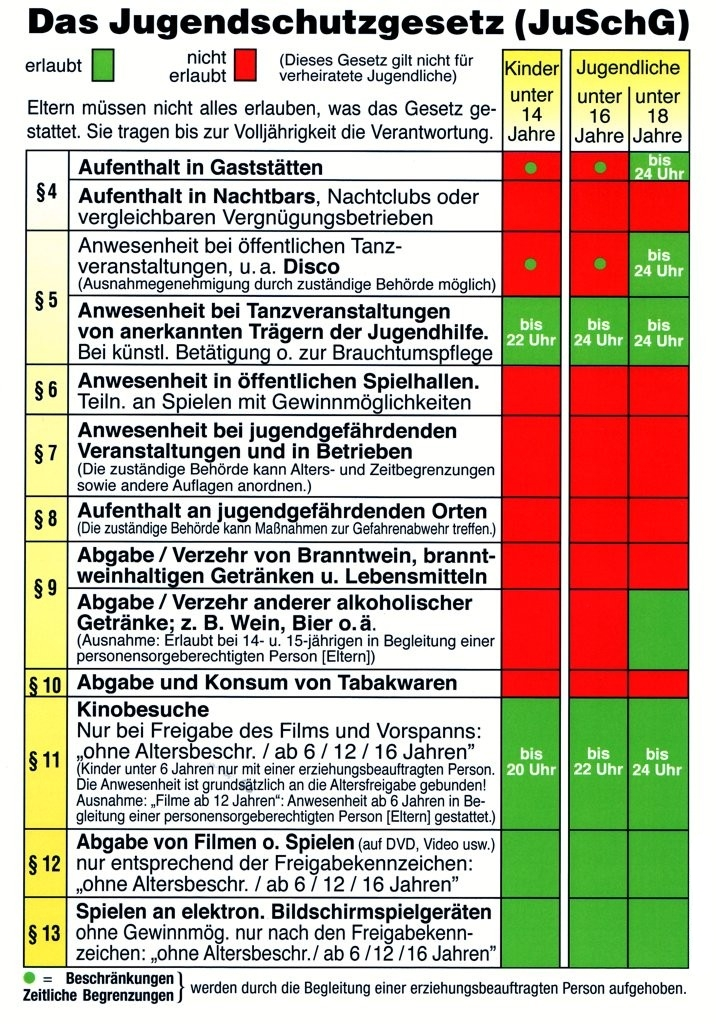
\includegraphics[width=8cm]{pic/js.jpg}
  \caption{Jugendschutzgesetz Bestimmungen.}
  \label{fig:js}
\end{figure}
\citetitle{theorie} Seite 134
\end{solution}
\section{Sportp"adagogik}
\begin{question}{4}
Diskutieren Sie den Begriff der Handlungsfa"ahigkeit im Schneesport.
\end{question}
\begin{solution}
Handlungsf"ahigkeit im engeren Sinne als praxisbezogener Begriff bezieht sich hier auf die spezifische Handlungsf"ahigkeit im Schneesport. Aufgrund der "au"seren Rahmenbedingungen (Outdoor, Skigebiet als Bewegungsraum u.a.) ben"otigen die Sch"uler ein bestimmtes Ma"s an motorischem K"onnen, konkrete sportartspezifische Kenntnisse (FIS-Regeln, Verhalten in der Gruppe, Orientierung im Gebiet u.a.) sowie die Bereitschaft, das Wissen und K"onnen auch tats"achlich anzuwenden. Der Erwerb von Kompetenzen soll die Sch"uler bef"ahigen, sicher, selbsta"andig und souver"an am Schneesport teilzunehmen.\\
Handlungsf"ahigkeit im weiteren Sinne hei"st nicht nur, die Sportart aus"uben zu k"onnen. Die Sch"uler sollen sich im Schneesport so gut auskennen, dass entscheiden k"onnen, was Schneesport f"ur sie bedeutet. Ziel ist, "uber die konkrete sportliche Aktivit"at hinaus, selbstbestimmt und m"undig zu entscheiden, was f"ur das eigene Leben relevant ist und damit die eigene Identit"at zu st"arken.\\\\
\citetitle{theorie} Seite 144
\end{solution}

\begin{question}{5}
Nennen Sie die grundlegenden Zielsetzungen im Schneesport aus sportp"adagogischer Sicht und erl"autern Sie diese jeweils anhand eines Beispiels. 
\end{question}
\begin{solution}
Ziele im Schneesport: bewegungsbezogenes Lernen und Pers"onlichkeitsentwicklung\\
Bewegungsbezogenes Lernen:
\begin{itemize}
\item Bewegungserfahrungen, die sich einer direkten Belehrung entziehen, in m"oglichst gro"ser Vielfalt zu f"ordern: subjektive Innenansicht der Bewegung
\item Bewegungsk"onnen anhand der sportartspezifischen Strukturen und grundlegenden Technikmerkmale einschlie"slich Kenntnissen "uber Aktions-Funktions-Zusammenh"ange vermitteln: objektive Au"senansicht der Bewegung
\item Bewegungsbezogene Einstellungen und Haltungen f"ordern, die eine intensive und ver- antwortungsvolle Auseinandersetzung mit Gegebenheiten und Herausforderungen im Schneesport unterst"utzen
\end{itemize}
Beispiel: Anhand Bewegungsmerkmale Bewegungsk"onnen verbessern.\\\\
Pers"onlichkeitsentwicklung aus p"adagogischer Sicht:
\begin{itemize}
\item Selbstbestimmung: Die Sch"uler sollen f"ur sich selbst Sinn in bestimmten Aktivit"aten oder situativen Gegebenheiten des Schneesports entdecken und entsprechende Entscheidungen treffen.
\item Mitbestimmung: Die Sch"uler k"onnen ihren eigenen Standpunkt, ihre Interessen und Bed"urfnisse, also ihre eigene Sinnfindung innerhalb der Gruppe kommunizieren und
vertreten.
\item Solidarit"at: Die Sch"uler k"onnen die Sinnfindungen anderer, also deren Standpunkte,
Interessen und Bed"urfnisse, anerkennen. Sie sind also kompromissbereit, zeigen Hilfsbereitschaft und treten aktiv f"ur andere Gruppenmitglieder ein.
\end{itemize}
Beispiel: "au"sern eigener Ideen zu neuen "ubungen (Mitbestimmung).\\\\
\citetitle{theorie} Seite 146-153
\end{solution}

\begin{question}{5}
Erl"autern Sie den Unterschied zwischen Au"sen- und Innensicht von Bewegungen. Diskutieren Sie den Einsatz im Unterricht. 
\end{question}
\begin{solution}
\emph{Objektive Au"senansicht:} Sicht auf die Bewegung anhand ihrer Struktur- und Technikmerkmale. Orientiert sich an den konkreten Merkmalen von Bewegungstechniken. Im Unterricht soll anhand der Bewegungsmerkmale und des Wissens "uber aktionale und funktionale Zusammenh"ange im situativen Bezug das Bewegungsk"onnen des Sch"ulers verbessert werden.\\
\emph{Subjektive Innenansicht:} Sicht des Sch"ulers seines sich Bewegens. Sp"uren von Bewegungserfahrungen (Erfahrungsqualit"aten). Bedingt durch die individuelle Auseinandersetzung mit der Umwelt. Im Unterricht soll das Erfahrungsspektrum erweitert werden.\\
\emph{Fazit:} Man sollte sich nicht zu stark im Unterricht an Technikleitbildern orientieren, jeder Sch"uler soll Technikmerkmale individuell umsetzen und mit seinen eigenen k"orperlichen Voraussetzungen in Einklang bringen. Das Bewegungslernen soll im Wechsel von technikorientiertem Bewegungsk"onnen und Bewegungserleben gestaltet sein.\\\\
\citetitle{theorie} Seite 147-149
\end{solution}

\begin{question}{6}
Nennen Sie die drei F"ahigkeiten zur Pers"onlichkeitsentwicklung und beschreiben Sie diese jeweils anhand eines Beispiels.
\end{question}
\begin{solution}
\emph{Selbstbestimmung:} Die Sch"uler sollen f"ur sich selbst Sinn in bestimmten Aktivit"aten oder situativen Gegebenheiten des Schneesports entdecken und entsprechende Entscheidungen treffen.
\emph{Mitbestimmung:} Die Sch"uler k"onnen ihren eigenen Standpunkt, ihre Interessen und Bed"urfnisse, also ihre eigene Sinnfindung innerhalb der Gruppe kommunizieren und vertreten.
\emph{Solidarit"at:} Die Sch"uler k"onnen die Sinnfindungen anderer, also deren Standpunkte, Interessen und Bed"urfnisse, anerkennen. Sie sind also kompromissbereit, zeigen Hilfsbereitschaft und treten aktiv f"ur andere Gruppenmitglieder ein.\\\\
\citetitle{theorie} Seite 151
\end{solution}

\begin{question}{6}
Was verstehen Sie unter reflexivem Lehren und Lernen?
\end{question}
\begin{solution}
Lernen soll reflexiv begleitet werden, um nachhaltig zu sein. Das Nachdenken "uber das Erlebte und dessen Thematisierung im Unterricht gilt als zentrales Element des Lernprozesses. Die Reflexion kann sich auf motorische Aspekte (Bewegungserlebnisse) und auf das psychische (Emotionen) und soziale Erleben (Erlebnisse im Austausch mit anderen) beziehen.\\
\emph{Schwerpunkte der Reflexion:}
\begin{itemize}
\item Die Selbstbeobachtung und Selbstwahrnehmung in aktuellen Situationen, sodass die Sch"uler f"ur das, was sie erleben, sensibilisiert werden.
\item Das Verst"andnis f"ur Zusammenh"ange und Abl"aufe. Warum passiert das was gerade geschieht?
\item Die Verkn"upfung des Erlebten mit fr"uheren Erfahrungen, um das Ereignis vor dem jeweils eigenen Erfahrungshorizont deuten und einordnen zu k"onnen. Dazu geh"ort auch die Verkn"upfung von neuem Wissen mit bereits bekannten Zusammenh"angen. 
\end{itemize}
\emph{Ziel der Reflexion:} Nachhaltiges Verstehen von Bewegungsph"anomenen ebenso wie von psychischen Aspekten und sozialen Ereignissen: Erproben und Verstehen und Einordnung in den Gesamtzusammenhang.\\\\
\citetitle{theorie} Seite 154
\end{solution}

\begin{question}{6}
Nennen Sie die physischen und psychosozialen Lernvoraussetzungen f"ur Sch"uler im Vorschulalter/ Schulkindalter/ in der Pubert"at/ im Erwachsenenalter.
\end{question}
\begin{solution}
Siehe Tabelle \ref{learning}.\\\\
\citetitle{theorie} Seite 156 - 163
\begin{table}
\caption{Lernvoraussetzungen in verschiedenen Altersstufen.}
  \label{learning}
  \scriptsize
  \begin{center}
    \begin{tabular}{p{2,5cm}|p{5,5cm}|p{5,5cm}}
      \textbf{Lernender} & \textbf{physische Lernvoraussetzungen} & \textbf{psychosoziale Lernvoaussetzungen}\\
    \hline
      Vorschulalter & 3-4 Jahre: Lernen von Bewegungsgrundformen; 4-6 Jahre: Ausdifferenzierung der Bewegungsgrundformen, Kombination von Bewegungen und Verbesserung der koordinativen F"ahigkeiten & Intensives Spiel- und Bewegungsbed"urfnis; Aufmerksamkeitsspanne ausgesprochen kurz; Im sozialen Kontakt noch stark auf sich selbst bezogen und teilweise von Gruppenspielen oder Partneraufgaben "uberfordert\\
      Schulkindalter (7J. bis Pubert"at) & Ver"anderung der K"orperproportionen; Sehr gute Last-Kraft- und Hebelverh"altnisse; Ideale Voraussetzungen f"ur das Bewegungslernen; Rasche Fortschritte in der motorischen Lernf"ahigkeit; goldenes Lernalter & Begeisterung und Entdeckerfreude k"onnen leicht in "ubermut und Unkontrolliertheit umschlagen; Spontanes und intuitives Lernen; Verbesserung der Konzentrationsf"ahigkeit und Reflexionsf"ahigkeit, Steigerung der kognitiven Leistungsf"ahigkeit; Entwicklung im Sozialverhalten: mit
sozialem Kontakt steigt das Empfinden f"ur die eigene Individualit"at\\
Pubert"at (M: 11/12 bis 13/15; J: 12/14 bis 15/17) & Gravierender Wachstumsschub, "anderung der gewohnten Proportionen; St"orung der Bewegungsabl"aufe, somit anpassen und neu lernen; Gewohnte Handlungsabl"aufe funktionieren u.U. nicht mehr, neue sind noch nicht stabilisiert; M"ogl. Stagnation des Bewegungslernens; Gro"se Unterschiede im physischen Entwicklungsstand & Ver"anderung des eigenen K"orpers irritiert; Unklare Rolle im sozialen Kontext: der Kindheit entwachsen, im Erwachsenenalter noch nicht wirklich angekommen, dadurch Verunsicherung, durch die das Erleben der eigenen Kompetenz sowohl in bewegungsbezogener als auch in pers"onlichkeitsbezogener Hinsicht reduziert sein kann; Starke Zunahme der intellektuellen F"ahigkeiten; Werden zunehmend selbst"andig; Teilzeit-Experten\\
Erwachsenenalter (Ab 18/20 Jahren) & Ca. 18-30/35 J.: Harmonisierung der k"orperlichen Proportionen, gleichbleibende K"orperproportionen und relativ konstante motorische Leistungsf"ahigkeit; zweites goldenes Lernalter; hohe physische Leistungsf"ahigkeit; Ab ca. 30/35 J.: Motorische Leistungsminderung & Psychische Ausgeglichenheit; Auseinandersetzung mit abnehmender Leistungsf"ahigkeit
    \end{tabular}
  \end{center}
\end{table}
\end{solution}

\begin{question}{4}
Nennen Sie verschiedene Rollen, die Sie als Schneesportlehrer einnehmen k"onnen. Beschreiben Sie eine davon. 
\end{question}
\begin{solution}
\emph{Rollen des Schneesportlehrers:}
\begin{itemize}
\item Lernbegleiter
\item Vorbild oder Modell
\item Ansprechpartner und Vertrauensperson
\item Organisator
\end{itemize}
\emph{Schneesportlehrer als Vorbild:}
Durch unser Verhalten bestimmen wir in gro"sem Ma"se mit, wie Sch"uler in bestimmten Situationen agieren, nicht zuletzt bedingt durch unseren Expertenstatus.\\
Der Skilehrer pr"asentiert sich permanent mit seinem Fahrk"onnen. Sch"uler lernen auch durch Nachahmung, daher spielt unser Fahrk"onnen f"ur das bewegungsbezogene Lernen eine gro"se Rolle.\\
In Bezug auf ein pers"onlichkeitsbezogenes Lernen orientieren sich unsere Sch"uler h"aufig an unserem Verhalten. Umgang mit Leistungsunterschieden in der Gruppe, Vermittlung von Erfolgserlebnissen, Umgang mit Konflikten.\\
Vorbildfunktion hinsichtlich weiterer handlungsrelevanter Kompetenzen im Schneesport: Verhalten im Skigebiet, Sicherheit etc.\\\\
\citetitle{theorie} Seite 163-172
\end{solution}

\begin{question}{6}
Nennen Sie die drei relevanten Aspekte f"ur das F"uhren von Gruppen und erl"autern Sie diese jeweils anhand eines Beispiels.
\end{question}
\begin{solution}
\emph{Verhalten:}\\
Verbales Verhalten: das gesprochene Wort, die Information, Zahlen, Daten, Fakten\\
Nonverbales Verhalten: Mimik, Gestik, K"orperhaltung, Blickkontakt\\
Paraverbales Verhalten: Lautst"arke, Sprechgeschwindigkeit, Sprachmelodie\\
Nonverbale und paraverbale Signale werden h"oher bewertet als die verbalen Signale.\\
Keine Doppelbotschaften senden, bei denen mehrere Signale im Widerspruch zueinander stehen, sondern klar und in den Signalen eindeutig sein.\\
Das gesprochene Wort muss gelebt werden!\\
\emph{Versuch:}\\
Durch Versuche entwickeln wir ein Gesp"ur f"ur die einzelnen Kursteilnehmer (unterschiedliche Lerntypen, jeweilige Motivation) und k"onnen auch die Ansprache individuell modifizieren.\\
\emph{Erfolg:}\\
Im Schneesport kann Erfolg sehr unterschiedlich aussehen, je nach Motivation und Ziel. Damit ist der Begriff bedeutungsoffen.\\
Wesentliche Aufgabe: Erfolg zusammen mit der Gruppe definieren und damit ein Ziel f"ur alle zu finden.\\\\
\citetitle{theorie} Seite 172-175
\end{solution}

\begin{question}{6}
Wie lautet die Definition von F"uhrung. Geben Sie je zwei Beispiele zur verbalen und nonverbalen F"uhrung von Personen im Unterricht Ihrer Disziplin.
\end{question}
\begin{solution}
F"uhrung ist die Art und Weise, wie ich mich verhalte, wenn ich versuche, andere zum Erfolg zu f"uhren.\\
Verbale F"uhrung: das gesprochene Wort, Zahlen, Daten, Fakten\\
Nonverbale F"uhrung: Mimik, Gestik, K"orperhaltung Blickkontakt\\\\
\citetitle{theorie} Seite 173
\end{solution}

\begin{question}{6}
Welche Phasen der Gruppenentwicklung nach Tuckman gibt es? Beschreiben Sie die Phase des Forming/ Storming/ Norming/ Performing/ Adjourning anhand eines Beispiels und einer Skizze.
\end{question}
\begin{solution}
\emph{Forming (Kennenlernen)}\\
F"ur das Gelingen des Kurses sehr wichtig, denn hier treffen die Teilnehmer mit ihren Werten, Einstellungen und Vorerfahrungen zum ersten Mal aufeinander.\\
Sch"uler sind auf Lehrkraft ausgerichtet und verhalten sich untereinander nett, tasten sich ab und versuchen ihren Platz in der Gruppe zu finden\\
Lehrer:\\
Vorgabe von Richtung und Struktur, Reglementierung der Verhaltensweisen, Regeln und Normen\\
Herstellung eines guten Kontakts zwischen Lehrer und Sch"ulern\\
Provokation und F"orderung der Kommunikation unter Sch"ulern\\ 
\emph{Storming (Machtkampf)}\\
Gruppenmitglieder sind bem"uht, Unterschiede hervorzuheben und sie suchen ihren Platz, ihre Rolle in der Gruppe. Dabei kann es zu Konkurrenz- oder Machtk"ampfen und Konflikten kommen.\\
Lehrer:\\
Klare und konsequente Einforderung der Einhaltung der Regeln\\
Lehrer als Moderator beobachtet und agiert prozessorientiert\\
Unterst"utzt die Sch"uler dabei, ihren Platz und ihre Rolle in der Gruppe zu finden\\
Sieht und wertsch"atzt individuelle Leistungen, somit individuelle Aufmerksamkeit\\
\emph{Norming (Vertrautheit)}\\
Die Beziehung zur Lehrkraft verliert an Bedeutung. Die Gruppe kommt allm"ahlich zum Laufen. Gruppe hat sich auf gemeinsame Regeln und Normen geeinigt. Teilnehmer akzeptieren ihre Rollen und f"ullen sie aus. Das Verhalten des Einzelnen wird damit f"ur die anderen einsch"atzbar und kalkulierbar. Das Vertrauen untereinander w"achst und es besteht die Chance auf ein Wir-Gef"uhl.\\
Lehrer:\\
In den Hintergrund treten und f"ur einen guten Rahmen sorgen\\
Mehr und mehr Verantwortung an die Gruppe abgeben 
\emph{Performing (Differenzierung)}\\
Die Zusammenarbeit der Gruppe verl"auft erfolgreich und ihre Mitglieder unterst"utzen sich gegenseitig.\\
Lehrer:\\
Aufrechterhaltung der vorhandenen positiven Gruppendynamik: Wie ein DJ, der es schafft, die Tanzfl"ache zu f"ullen, braucht der Lehrer nun einen Sp"ursinn daf"ur, was die Gruppe gerade braucht. Wir m"ussen mit verschiedenen "ubungen, Aufgaben etc. das bieten, was die Gruppe gerade will.\\
Moderator und Impulsgeber\\
\emph{Adjourning (Abl"osung)}\\
Teilnehmer orientieren sich neu, weg von der Gruppe\\
Lehrer hat die Aufgabe, den Prozess des Abschieds zu steuern\\\\
\citetitle{theorie} Seite 173 - 186
\end{solution}

\begin{question}{6}
Erl"autern Sie den Unterschied zwischen einer Gruppe und einem Team.
\end{question}
\begin{solution}
Ein Team ist eine Gruppe von Personen mit komplement"aren F"ahigkeiten, die f"ur einen ge- meinsamen Zweck und eine Reihe spezifischer Leistungsziele eingesetzt werden. Mitglieder haben sich verpflichtet, miteinander zu arbeiten, um das gemeinsame Ziel zu erreichen, und tragen Verantwortung f"ur die Ergebnisse des Teams.\\
Als Lehrkr"afte m"ussen wir uns gut "uberlegen, ob wir eine funktionierende Gruppe oder ein Team ben"otigen, um ein bestimmtes Ziel zu erreichen. F"ur einen gew"ohnlichen Skikurs ist es sicherlich schon sehr gut, wenn die Gruppe die Performing-Phase erreicht.\\\\
\citetitle{theorie} Seite 184
\end{solution}

\begin{question}{3}
Nennen Sie 6 Regeln zur F"orderung einer positiven Gruppendynamik.
\end{question}
\begin{solution}
\begin{itemize}
\item Alle Mitglieder haben Anspruch darauf, ernst genommen zu werden.
\item Wir sprechen laut und deutlich, sodass alle uns verstehen k"onnen.
\item Der Ton macht die Musik. Wir pr"ufen, in welcher Stimmung wir vor die Gruppe treten.
\item Wir achten nicht nur auf unsere Sprache, sondern auch auf Mimik und Gestik.
\item Wir signalisieren unseren Gruppenmitgliedern, dass wir zuh"oren und sie verstehen. Dabei verwenden wir von ihnen benutzte Worte, wiederholen ihre Aussagen, erinnern an die morgens beim Start ge"au"serten Erwartungen.
\item Wir helfen den anderen, sagen aber auch, wenn wir selbst Hilfe brauchen.
\item Wir arbeiten mit Abschiedsritualen.
\end{itemize}
\citetitle{theorie} Seite 188
\end{solution}

\begin{question}{4}
Wie zeigen Sie echtes Interesse an den Teilnehmern? Welchen Effekt hat das auf den Teilnehmer?
\end{question}
\begin{solution}
\emph{Interesse Zeigen:}
\begin{itemize}
\item Aufmerksames Zuh"oren
\item Teilnehmer ernst nehmen
\item Keine missverst"andlichen Botschaften senden
\item Neugierig sein und Teilnehmer nach Hobbies, Beruf etc. fragen
\item Richtige Sprach- und Bildebene
\item Lernen, wie die Teilnehmer ticken und welche Ansprache sie brauchen
\item Lernen mit welchen methodischen Grunds"atzen und Verfahren wir die Teilnehmer locken k"onnen
\end{itemize}
\emph{Effekt:}\\
Bessere Gruppendynamik, Bessere Lernatmosph"are, Echtes Interesse vermittelt Vertrautheit - Leichteres Lernen f"ur den Teilnehmer\\\\
\citetitle{theorie} Seite 184
\end{solution}
\section{Sportdidaktik}
\begin{question}{4}
Nennen und beschreiben Sie vier didaktische Prinzipien f"ur die Gestaltung des Schneesportunterrichts.
\end{question}
\begin{solution}
Unterricht sollte:
\begin{itemize}
\item erfahrungsorientiert sein: Wir erkl"aren unseren Sch"ulern Zusammenh"ange nicht nur, sondern bieten ihnen Gelegenheiten, sie auch zu erleben und zu ersp"uren.
\item handlungsorientiert sein: Wir sorgen f"ur Lernsituationen, in denen die Sch"uler selbst t"atig sein k"onnen (z.B. bei der Wahl der Pisten, der Organisation in der Gruppe, dem Umgang mit dem Material usw.)
\item individualisiert sein: Wir gehen auf jeden Sch"uler mit seinen jeweiligen Voraussetzungen und Entwicklungszielen ein.
\item reflexiv sein: Wir sprechen mit den Sch"ulern "uber Erlebtes und regen zum Nachdenken dar"uber an.
\end{itemize}
\citetitle{theorie} Seite 197
\end{solution}

\begin{question}{3}
Welche personalen / materialen Voraussetzungen ber"ucksichtigen Sie im Schneesportunterricht? 
\end{question}
\begin{solution}
\emph{Personale Voraussetzungen:}\\
Individuelle Voraussetzungen der Sch"uler: Alter und Entwicklungsstand; Aktuelles schneesportliches K"onnen und Wissen; Einstellungen und Haltungen in Bezug auf bewegungsorientierte Aktivit"aten; Interessen und W"unsche\\
Voraussetzungen der Gruppe: Wie funktioniert die Gruppe im Zu- sammenspiel/ als Einheit? Beeinflusst Unterrichtsmethoden, Inhalte, Fahrtempo etc.\\
Schneesportlehrer: Eigene Voraussetzungen – Wissen und K"onnen, Einstellungen und Haltungen, Interessen und W"unsche; bestimmen den Unterricht grundlegend mit; Gepr"agt durch Vorerfahrungen, die zu unserem pers"onlichen Verst"andnis vom Schneesport f"uhren und bestimmen, was wir wie an unsere Sch"uler weitergeben wollen.\\
\emph{Materielle Voraussetzungen:}\\
Gel"ande- und Schneeverh"altnisse; Wetterverh"altnisse; Ausr"ustung\\\\
\citetitle{theorie} Seite 199-211
\end{solution}

\begin{question}{8}
Nennen Sie drei Unterrichtsverfahren zur Steuerung im Unterricht und deren Merkmale (mindestens drei). Geben Sie zu einem Verfahren ein praktisches Beispiel aus ihrer Disziplin.
\end{question}
\begin{solution}
\emph{Direkte Steuerung:}\\
Schneesportlehrer als Instrukteur; F"uhrt Regie im Unterricht; W"ahlt Ziele und Inhalte aus; Nimmt Einteilung sinnvoller Lerneinheiten vor; Sorgt f"ur klares, strukturiertes, systematisches Vorgehen; Ber"ucksichtigt individuelle Differenzierung und Selbst"andigkeit der Sch"uler\\
Beispiel: Der Schneesportlehrer stellt mehrere aufeinander aufbauende Aufgaben zum Befahren einer Wellenbahn (Befahren in der Falllinie mit Beugen der Beine auf der Welle, Anfahrt in Schr"agfahrt mit Beugen auf der Welle etc.). Er erl"autert den Sch"ulern Aktions-Funktions- Zusammenh"ange und jeweils denn Sinn der Aufgabe. Er beobachtet die Sch"ulerfahrten im Umlaufbetrieb und gibt jedem Sch"uler nach seiner Fahrt ein Feedback zum Bewegungsablauf.\\
\emph{Kooperative Steuerung:}\\
Ziele und Inhalte werden nicht endg"ultig vom Schneesportlehrer festgelegt; Lehrer bringt Themen und Inhalte ein, die verhandelbar sind; Sch"uler handeln aus Forscherdrang, Neugier, Interesse und Motivation durch selbst initiiertes Probleml"osen; Lehrer sorgt f"ur Rahmen und Gelegenheiten, das Gelernte und Erfahrene selbstst"andig und vielseitig einzusetzen\\
Beispiel: Der Schneesportlehrer gibt das Thema bekannt und l"asst die Sch"uler in einer Fahrt in der Falllinie der Wellenbahn testen. Die Sch"uler bringen Ideen ein, welche Bewegungen zum Befahren sinnvoll sein k"onnten. Die Ideen werden erprobt und die Effekte verschiedener L"osungen kurz besprochen. In weiteren Fahrten werden auf Vorschlag des Lehrers und/oder Sch"ulers weitere Aspekte ver"andert, z.B. der Anfahrtswinkel auf die Welle oder das Fahrtempo. Ein kurzes Abschlussgespr"ach fasst die Bewegungserlebnisse zusammen.\\
\emph{Indirekte Steuerung:}\\
Schneesportlehrer gestaltet Lernumgebungen anhand von Gel"andewahl, Materialien und Aufgaben; Die Sch"uler lernen anhand authentischer Probleme un verschiedenen Kontexten; Die Sch"uler lernen im sozialen Austausch\\
Beispiel: Der Schneesportlehrer l"asst die Sch"uler eine Wellenbahn im Umlaufbetrieb befahren. Er ermuntert zu testen, wie es am besten geht bzw. welche unterschiedlichen Bewegungsm"oglichkeiten es gibt. Nach einigen Fahrten l"asst er die Sch"uler mit einem Partner Trainingsteams bilden. Die Paare sprechen bei jedem Durchgang ab, was sie nun ausprobieren wollen. Nach einigen Fahrten stellt der Lehrer Richtungstore auf die Wellen, die zu umfahren sind. Etwas sp"ater ver"andert er deren Position noch weiter aus der Falllinie heraus. Zum Abschluss werden die Varianten und die resultierenden Bewegungserlebnisse besprochen.\\\\
\citetitle{theorie} Seite 218-219
\end{solution}

\begin{question}{4}
Beschreiben Sie jeweils ein Beispiel f"ur eine M"undliche und Schriftliche Reflexion der Unterrichtsinhalte. 
\end{question}
\begin{solution}
\emph{Mündliche Reflexion:} Drei Smileys in den Schnee legen und dann Fragen zu den verschiedenen Ereignissen des Tages stellen. Die Sch"uler laufen bei jeder Frage zu dem Smiley, der ihrer Antwort entspricht.\\
\emph{Schriftliche Reflexion:} Schüler bekommen zu beginn ein Trainingstagebuch, in das sie verschiedene sachen eintragen können. Bestimmte Inhalte sind vorgegeben (Ziele, Selbsteinschätzzungen).\\\\
\citetitle{theorie} Seite 228-229
\end{solution}

\begin{question}{4}
Welche Aspekte der verbalen und nonverbalen Kommunikation ber"ucksichtigen Sie im Schneesportunterricht in der Altersstufe 4-7 Jahre /7-10 Jahre/ 10-12 Jahre/ 12-15 Jahre/ ab 15 Jahre.
\end{question}
\begin{solution}
\emph{Ab 4:}
\begin{itemize}
\item Kinder reagieren stark auf K"orpersprache. Nonverbales ist oft wichtiger als Worte. Al- so: Viel Wert auf Mimik und Gestik legen!
\item Blickkontakt w"ahrend des Gespr"achs ist in diesem Alter nicht so wichtig wie in ande- ren Altersgruppen. Wir sollten nur die Aufmerksamkeit der Kinder sicherstellen.
\item Die Kinder haben eine sehr kurze Aufmerksamkeitsspanne, deshalb kurze S"atze und einfache W"orter verwenden. Gespr"ache mit einzelnen Kindern sollten nur kurz sein.
\item Bei der Formulierung helfen, wenn den Kindern W"orter fehlen. Aber unbedingt nach- fragen, ob unsere Erg"anzung stimmt!
\item Fragen umformulieren und wiederholen, wenn das Kind eine Frage nicht versteht.
\item Bildhafte Sprache und phantasiereiche (Bewegungs-)Geschichten einsetzen.
\item Auf Augenh"ohe kommunizieren schafft N"ahe.
\end{itemize}
\emph{Ab 7:}
\begin{itemize}
\item Wir verwenden weiterhin bildhafte Sprache und phantasiereiche Geschichten.
\item Durch einen Sprung in der kognitiven Entwicklung (Lesen und Schreiben, abstraktes Denken) wird kindgerechtes Erkl"aren funktionaler Zusammenh"ange m"oglich.
\item Ironische Aussagen werden oft nicht verstanden.
\item Bei der Formulierung helfen, wenn den Kindern W"orter fehlen. Aber unbedingt nach- fragen, ob unsere Erg"anzung stimmt!
\item Materielle Belohnungen (eine besondere Abfahrt aussuchen d"urfen, Gummib"archen
etc.) stehen im Vordergrund, die Bedeutung immaterieller Belohnung (Wertsch"atzung
durch uns und Mitsch"uler) nimmt jedoch zu.
\end{itemize}
\emph{Ab 10:}
\begin{itemize}
\item Konkrete Erkl"arungen sind m"oglich, schwierige W"orter m"ussen wir erl"autern, bildhafte Sprache als Variante bzw. Untermalung einsetzen.
\item Erkl"arungen funktioneller Zusammenh"ange werden verstanden und sind sinnvoll, aber die Freude am Ausprobieren "uberwiegt.
\item Langatmige Erkl"arungen langweilen.
\item Die Meinung der gleichaltrigen ist ein wichtiger Ma"sstab, die soziale Akzeptanz spielt eine gro"se Rolle.
\item Die Bedeutung materieller Belohnungen nimmt ab (wird aber immer noch gesch"atzt), die Bedeutung immaterieller Belohnung (Lob/Anerkennung durch Erwachsene und Gleichaltrige) wird sehr gro"s.
\end{itemize}
\emph{Ab 12:}
\begin{itemize}
\item Die intellektuellen F"ahigkeiten nehmen stark zu, Jugendliche denken "uber vieles nach.
\item Heranf"uhren an die Fachsprache (insbes. im Leistungssport).
\item Fachsprache nutzen, aber mit Alternativbegriffen begleiten.
\item Jugendliche wollen nicht belehrt werden. Fragen stellen und die Gruppe gemeinsam an einer Sache arbeiten lassen, funktioniert besser.
\item Die Betonung auf Neues entdecken und ausprobieren ist hier genauso Gewinn bringend wie bei Kindern, um das Interesse wach zu halten.
\item Jugendliche wollen ernst genommen werden. Wenn wir ihnen eine Frage stellen, soll-
ten wir uns auch f"ur die Antwort interessieren.
\item Anerkennung durch Gleichaltrige steht im Zentrum.
\item Die Kommunikation zwischen Gleichaltrigen ist sehr intensiv, gegen"uber Erwachse-
nen deutlich zur"uckhaltender.
\item K"orpersprache verr"at vieles, was verbal nicht mitgeteilt wird, v.a. Unsicherheiten.
\end{itemize}
\emph{Ab 15:}
\begin{itemize}
\item Wir f"uhren Fachsprache ein und nutzen sie anschlie"send.
\item Unsere Aussagen sollten klar verst"andlich, pr"azise und informativ sein.
\item Aktives Zuh"oren zeigt Verbindlichkeit (non-verbal: z.B. Augenkontakt, Kopfnicken; verbal: z.B. Nachfragen, Kommentieren, Sch"uleraussagen in eigene Ansagen einbeziehen).
\item Wir sind als Experten gefragt und "uberzeugen v.a. durch unsere freundlich vermittelte
Fachkompetenz.
\item Wir betreuen individuell und vermitteln auch das entsprechende Gef"uhl.
\item Nonverbale Botschaften der Sch"uler dienen als wichtige Informationsquelle in Bezug auf Dinge, die im Rahmen der Gruppe aufgrund sozialer Gepflogenheiten evtl. nicht ge"au"sert werden.
\end{itemize}
\citetitle{theorie} Seite 234-236
\end{solution}
\section{Sportpsychologie}

\begin{question}{3}
Definieren Sie den Begriff der Sportpsychologie und nennen Sie die Ziele der Sportpsychologie im Schneesport.
\end{question}
\begin{solution}
Die Sportpsychologie befasst sich mit dem Verhalten und Erleben im Rahmen sportlicher Aktivit"at. Sie ist darauf gerichtet, dieses Verhalten und Erleben zu beschreiben, zu erklären, zu beeinflussen und das gewonnene Wissen praktisch anzuwenden.\\
\emph{Leistungssport:} Optimierung des Ablaufs sportlicher (H"ochst-)Leistungen im Wettkampf\\
\emph{Breitensport:} Unterst"utzung sportbezogener Lernprozesse und F"orderung von Spa"s am Schneesport\\\\
\citetitle{theorie} Seite 248
\end{solution}

\begin{question}{4}
Beschreiben Sie Faktoren, die das Lernklima im Unterricht beeinflussen und kennzeichnen Sie die Faktoren f"ur ein positives Lernklima.
\end{question}
\begin{solution}
\emph{Faktoren}
\begin{itemize}
\item Ad"aquate Aufgabenstellung zur Vermeidung von "Uber- oder Unterforderung
\item Angst als Gegner des Lernen (Aufbau von Selbstvertrauen und Umgang mit Angst)
\item Gruppenklima und Gruppenzusammenhalt (gute Stimmung und gegenseitige Unter-
st"utzung)
\item F"uhrungsstil des Skilehrers
\end{itemize}
\emph{Positives Lernklima:} Aufgabenstellung sehr wichtig. Eher aufgabenorientiertes (individuelle Bem"uhen der Sch"uler im Vordergrund), als wettbewerbsorientiertes (Leistungsvergleich im Vordergrund) Klima.\\\\
\citetitle{theorie} Seite 249-250
\end{solution}

\begin{question}{4}
Skizzieren Sie den Prozess der Kommunikation und nennen Sie vier Einflussfaktoren auf diesen.
\end{question}
\begin{solution}
\begin{figure}[H]
  \centering
  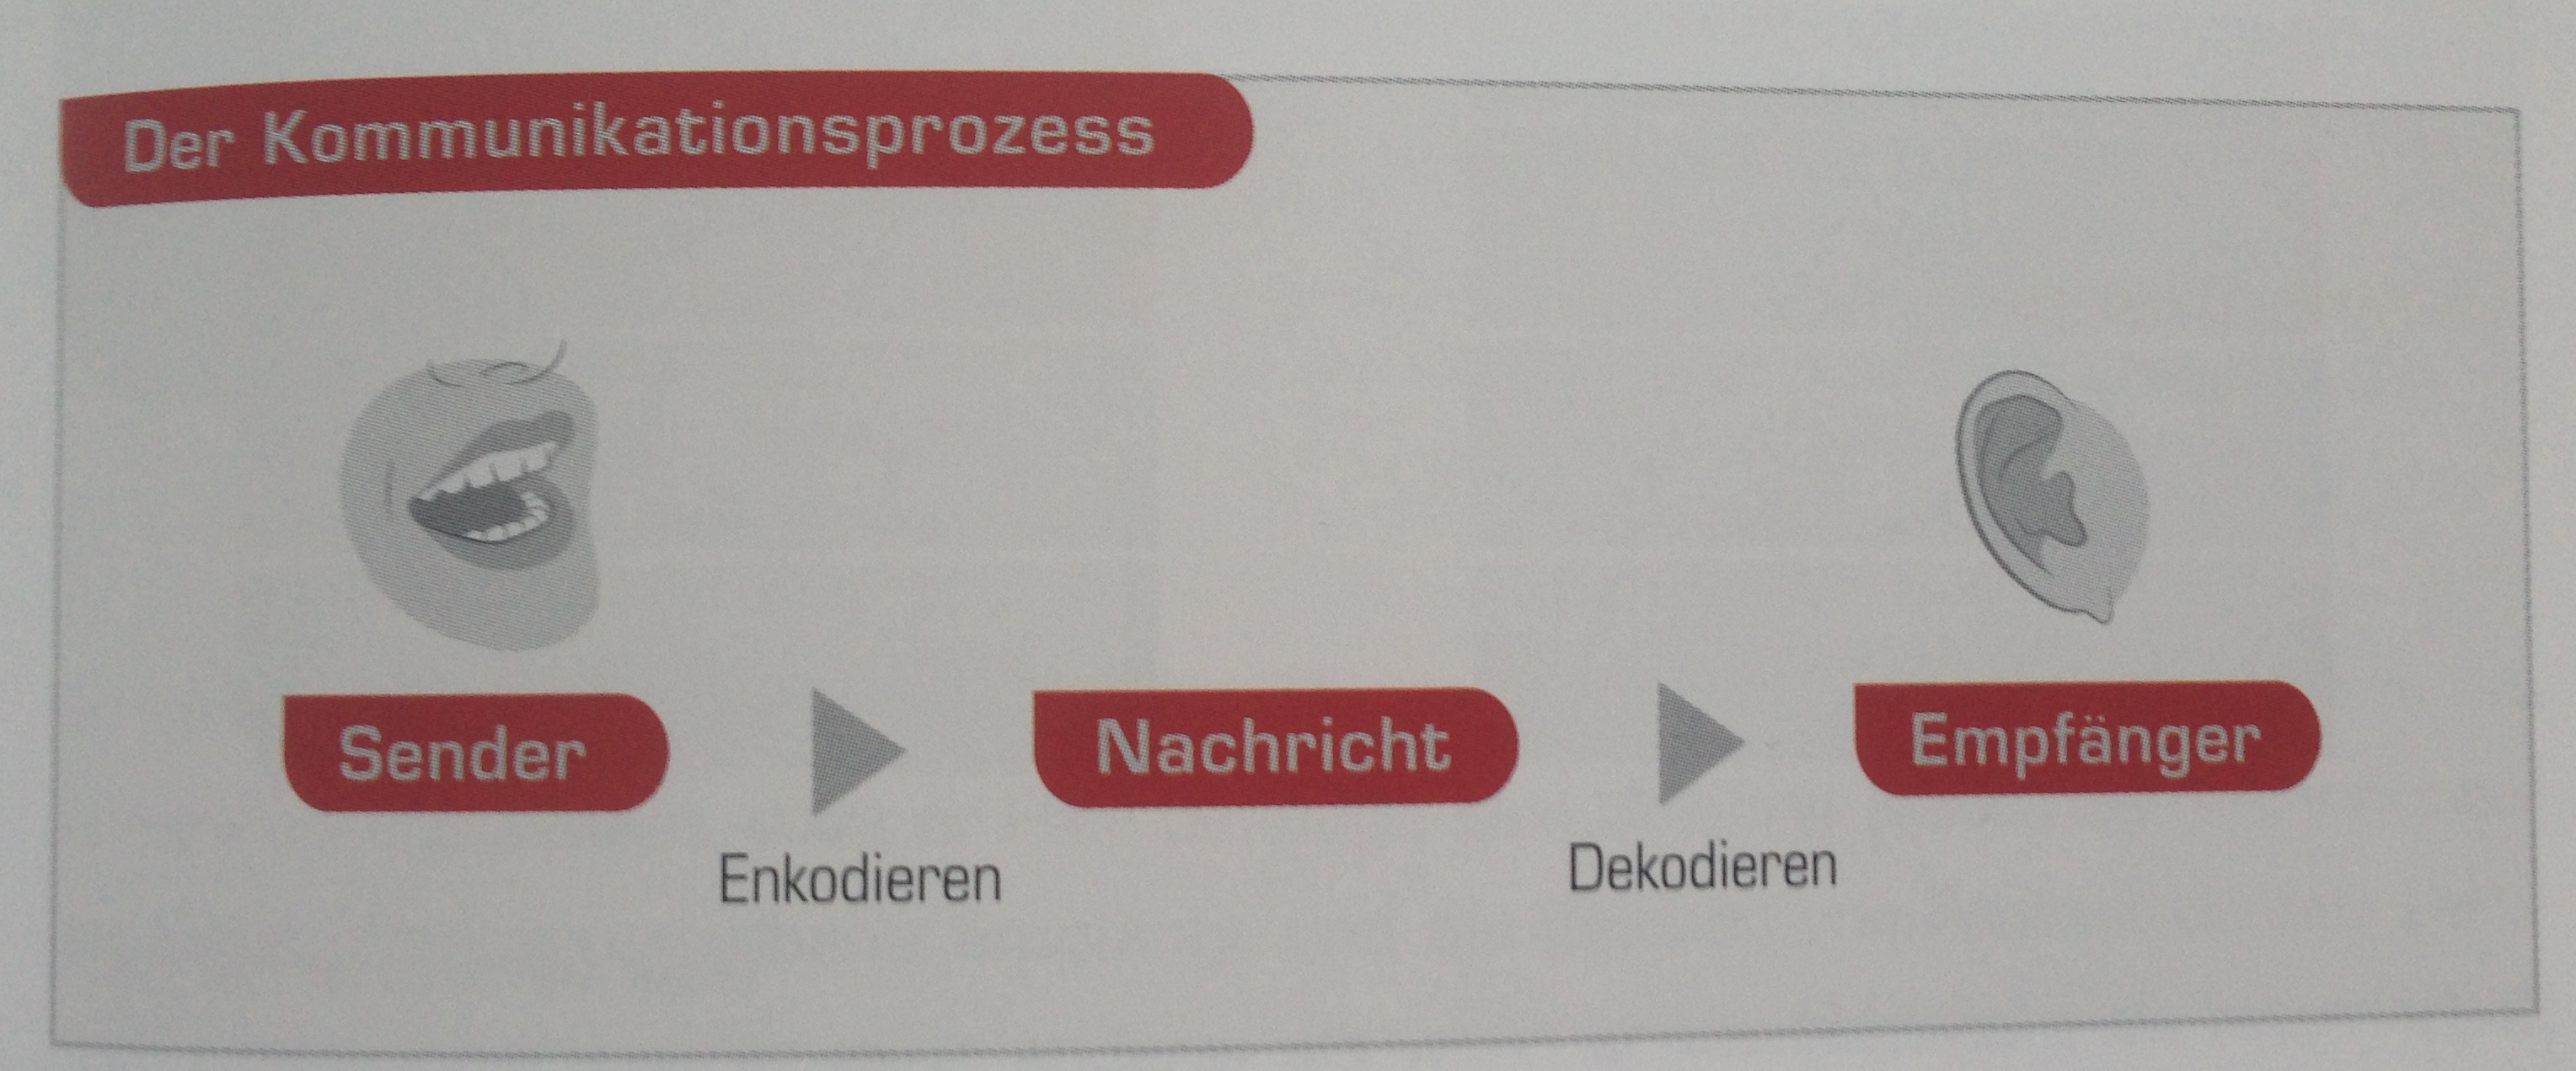
\includegraphics[width=12cm]{pic/kommunikation.jpg}
  \caption{Kommunikation.}
  \label{fig:kommunikation}
\end{figure}
\emph{Einflussfaktoren:}
\begin{itemize}
\item Aktuelle Stimmung und Emotionen
\item Erwartungen von Sender und Empfänger
\item Das gemeinsame Wissen (Verstehen Sender und Empfänger die gleichen Dinge unter den gleichen Begriffen?)
\item Aufmerksamkeit und Interesse
\item Zuf"allige Umst"ande
\item St"orungen wie z.B. Wind oder Betrieb auf der Piste
\end{itemize}
\citetitle{theorie} Seite 251-252
\end{solution}

\begin{question}{6}
Beschreiben Sie das Vier-Ohren-Modell der Kommunikation anhand eines Beispiels aus dem Schneesport.
\end{question}
\begin{solution}
\begin{figure}[H]
  \centering
  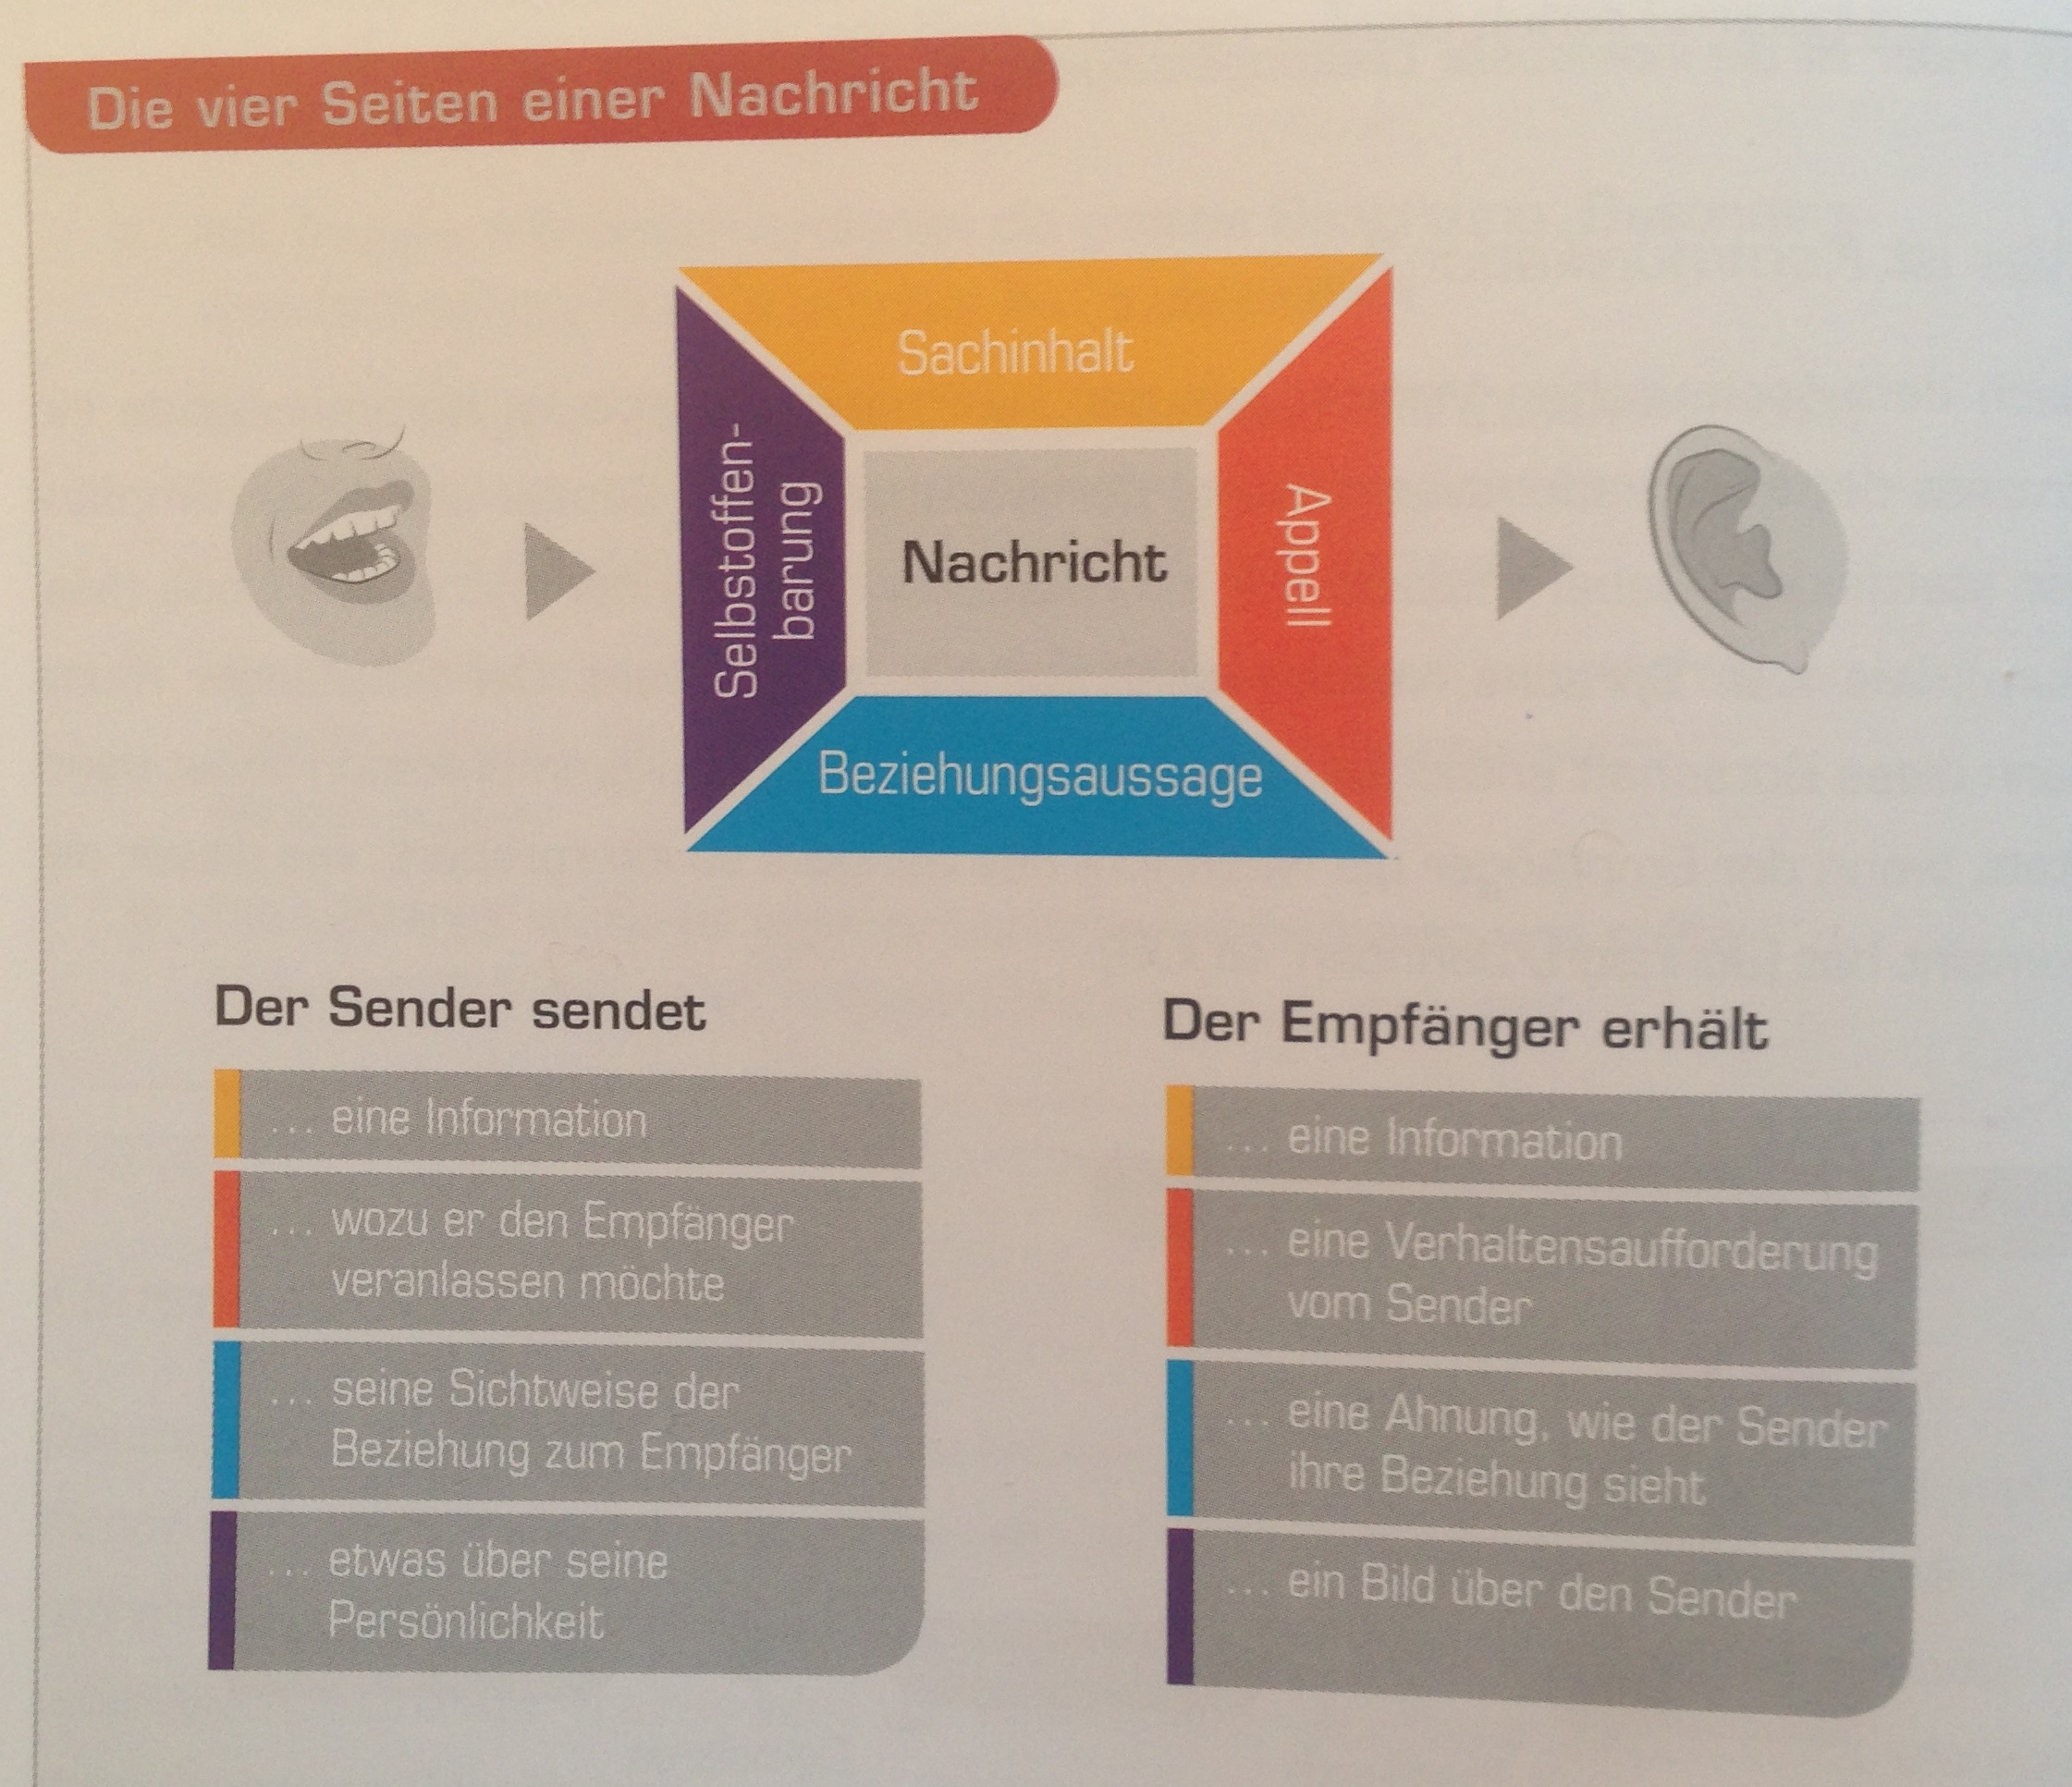
\includegraphics[width=12cm]{pic/vierohren.jpg}
  \caption{Vier Ohren Modell.}
  \label{fig:vierohren}
\end{figure}
\begin{figure}[H]
  \centering
  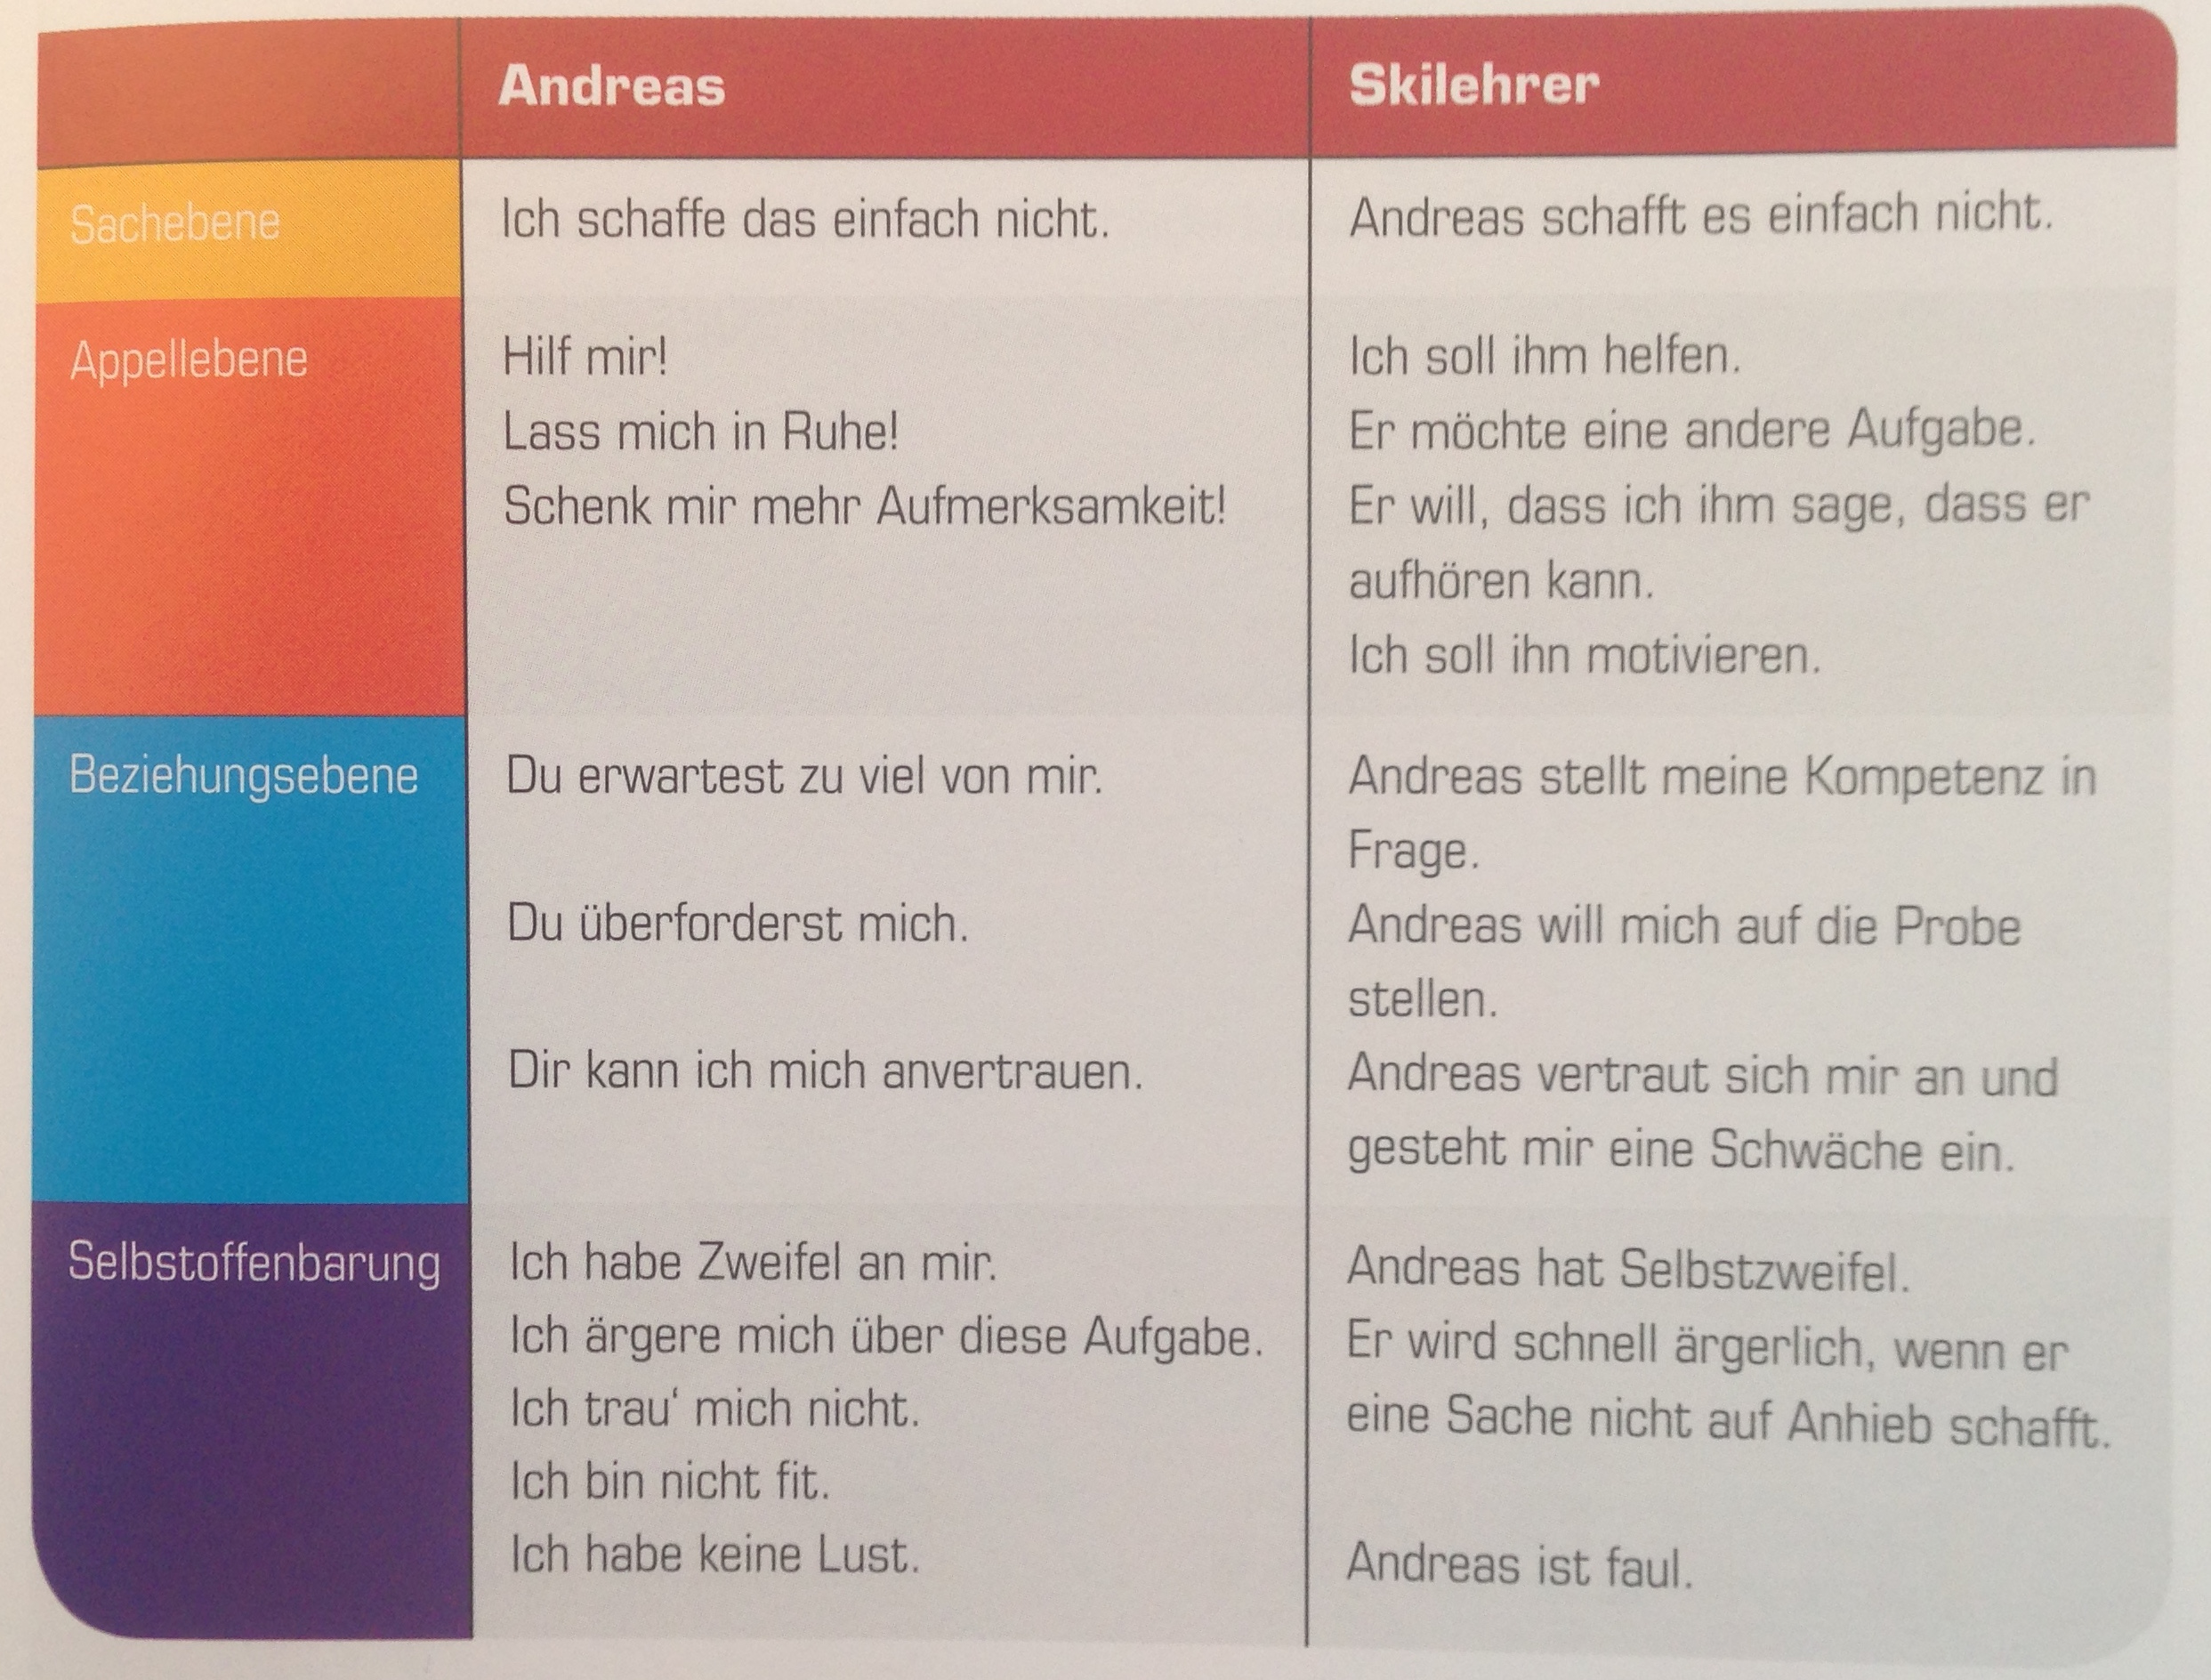
\includegraphics[width=12cm]{pic/vierohrenbsp.jpg}
  \caption{Beispiel.}
  \label{fig:viewrohrenbsp}
\end{figure}
\citetitle{theorie} Seite 252-253
\end{solution}

\begin{question}{6}
Als Schneesportlehrer müssen Sie f"ur eine erfolgreiche Kommunikation aktiv Zuh"oren. Wie setzen Sie dies konkret im Unterricht um?
\end{question}
\begin{solution}
\begin{figure}[H]
  \centering
  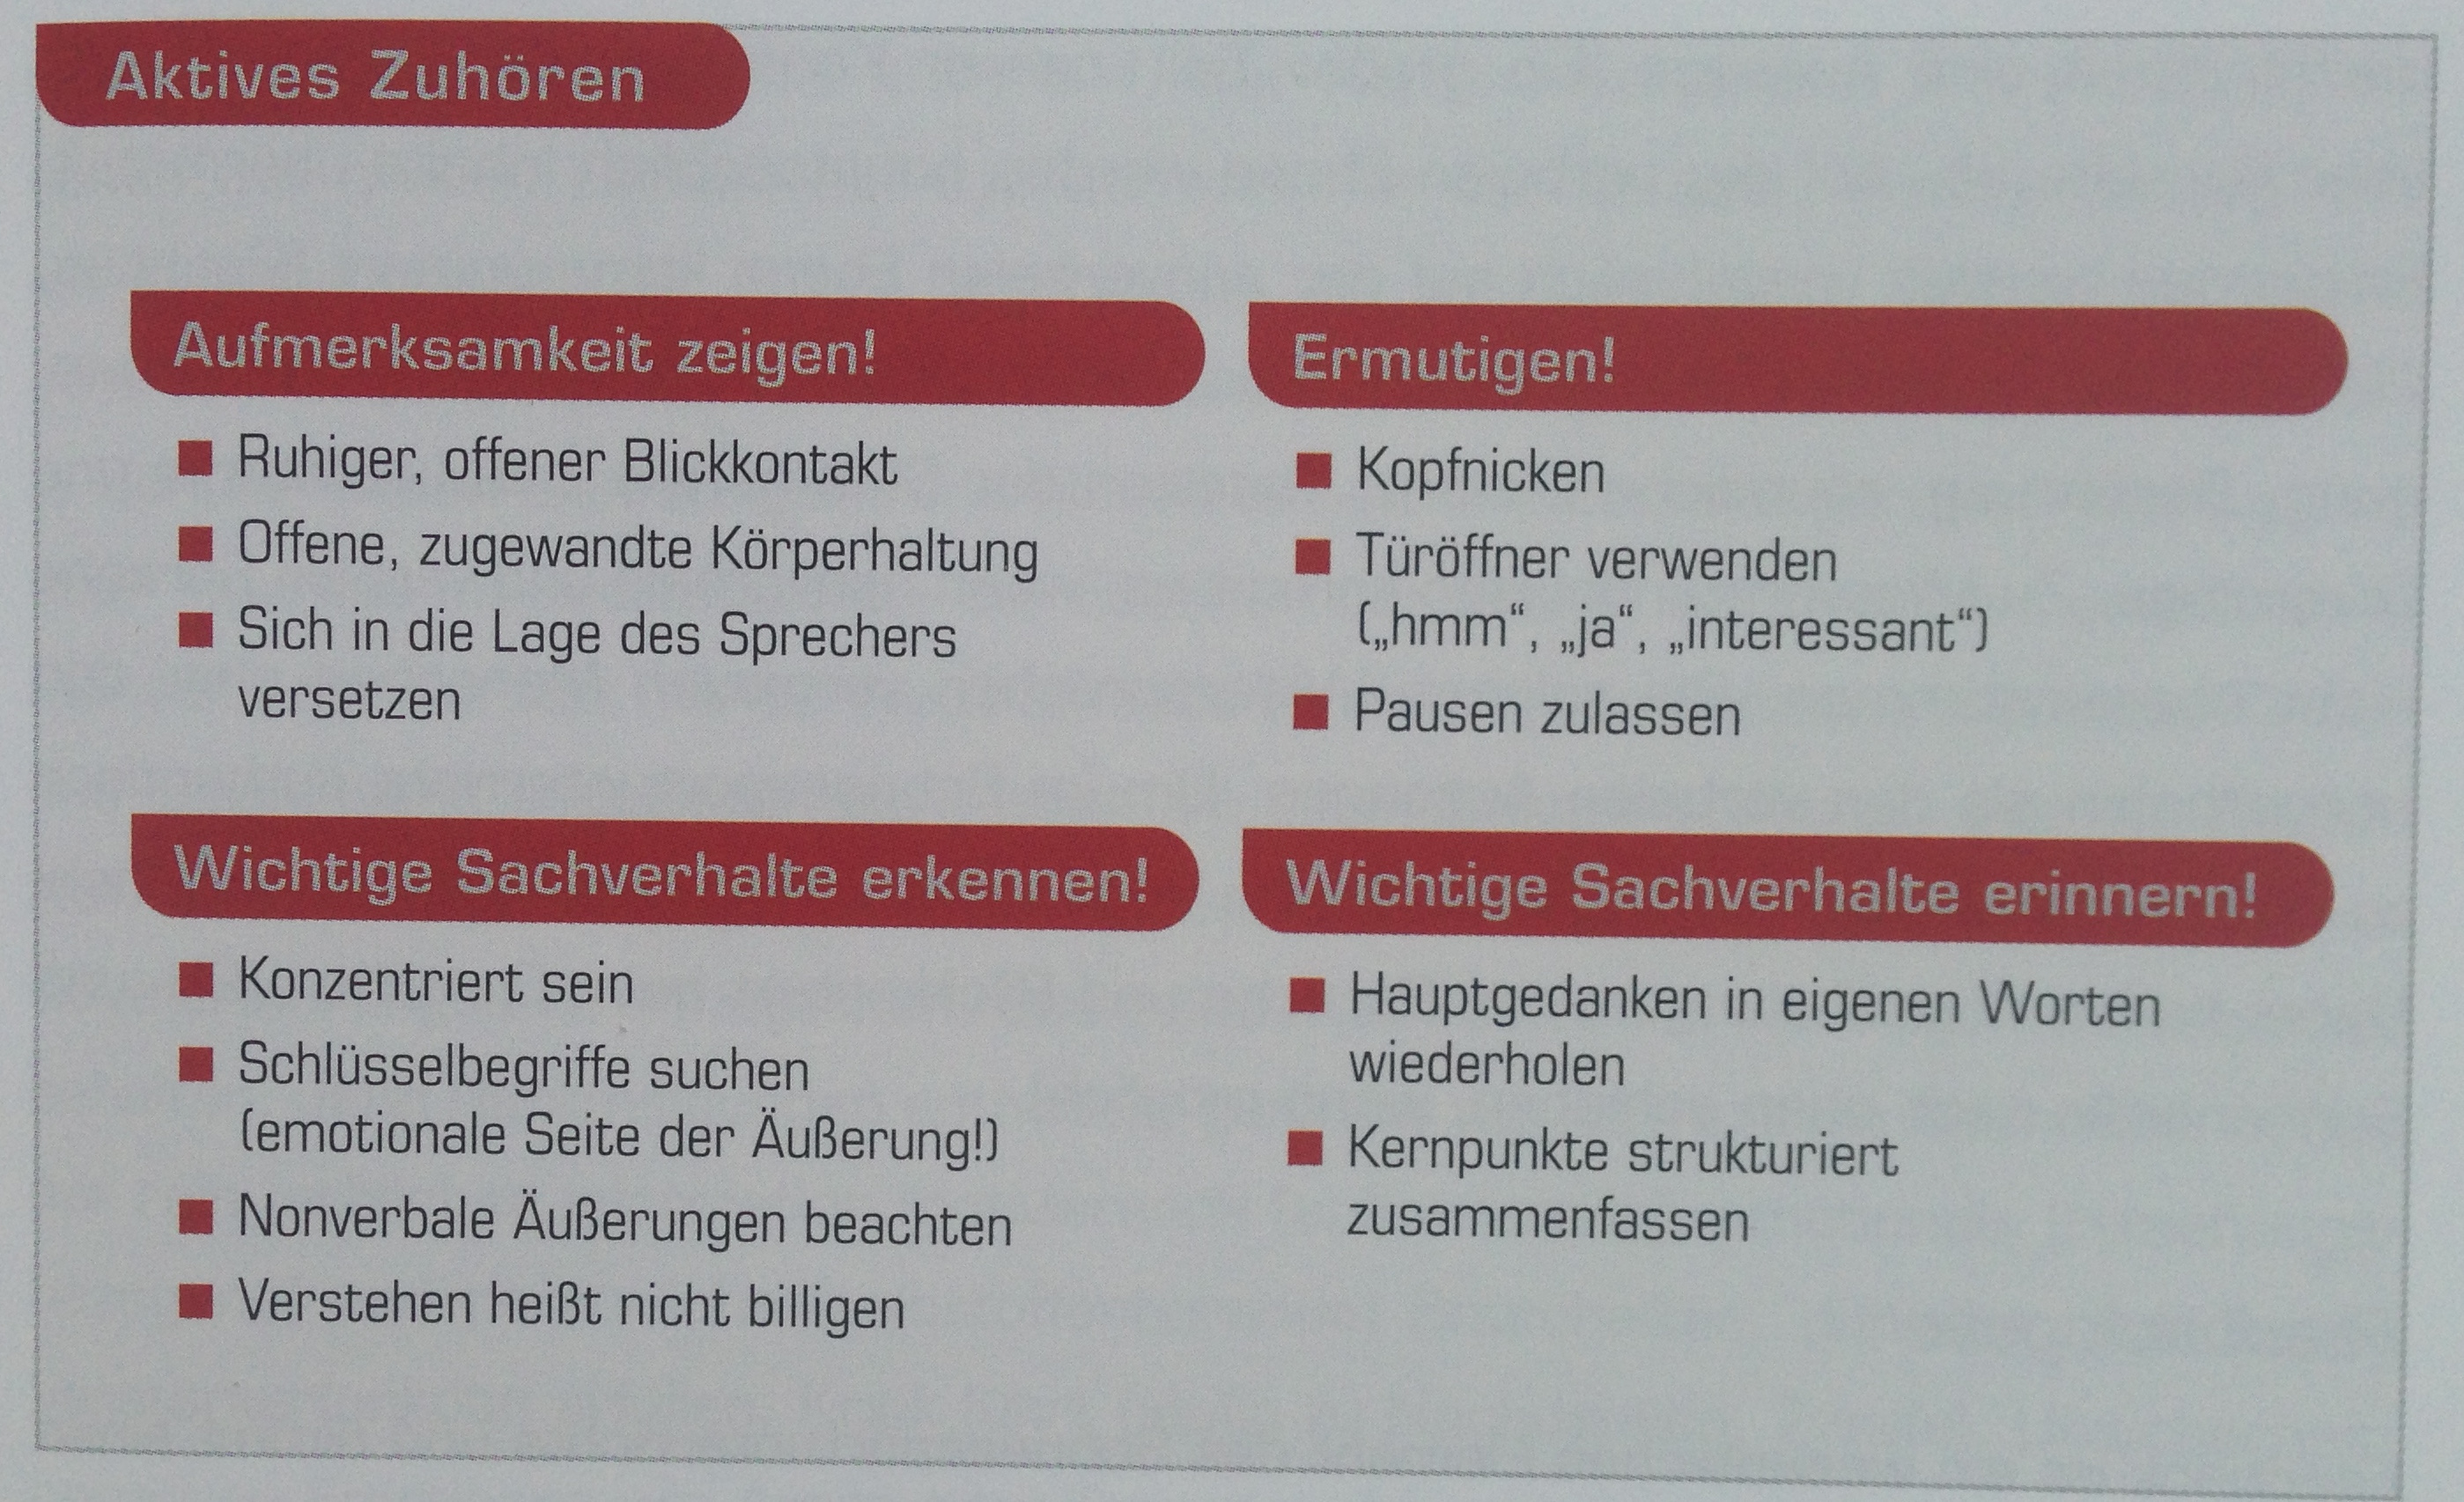
\includegraphics[width=12cm]{pic/zuhoeren.jpg}
  \caption{Aktives Zuhören.}
  \label{fig:zuhoeren}
\end{figure}
\citetitle{theorie} Seite 255
\end{solution}

\begin{question}{6}
Wie geben Sie Feedback an Ihre Sch"uler? Beschreiben Sie in diesem Zusammenhang f"unf Feedbackregeln.
\end{question}
\begin{solution}
\emph{Feedbackregeln}
\begin{itemize}
\item Als pers"onliche Wahrnehmung in Ich-Form: Ich habe gesehen, dass du rhythmisch und fließend gefahren bist., statt: Du fährst rhythmisch und fließend
\item Situationsbezogen: Bei dieser Fahrt hast du den Außenski wenig belastet., statt: Deine Außenskibelastung ist immer zu schwach.
\item Beschreibend ohne Wertung: Gerade bist du in R"uckenlage gefahren, statt: Du h"angst hinten drin, das ist schlecht.
\item Bezogen auf ver"anderbares Verhalten. Kritisiert wird nur das Verhalten, nicht die Person: Du sprichst zu laut., statt Du bist zu laut.
\item An den Bed"urfnissen des Sch"ulers ausgerichtet: f"ur Einsteiger h"aufiger, f"ur Fortgeschrittene seltener
\item Immer mit einem positiven Aspekt beginnen.
\end{itemize}
\citetitle{theorie} Seite 257
\end{solution}

\begin{question}{5}
Warum k"onnen zwischen Lehrer und Sch"uler Probleme bei der Kommunikation auftreten? Welche Ursachen k"onnen hierf"ur grunds"atzlich vorhanden sein?
\end{question}
\begin{solution}
\emph{Zwischen Kan"alen:} Wenn Lehrer und Sch"uler auf unterschiedlichen Kan"alen senden und Empfangen.\\
\emph{Innerhalb eines Kanals:} Beeintr"achtigungen auf Beziehungsebene (Streit)\\
St"orungen von Außen, Aufmerksamkeit, Interesse, Unterschiedliche Ausdrucksweise oder Sprache\\\\
\citetitle{theorie} Seite 252-257
\end{solution}

\begin{question}{4}
Definieren Sie den Begriff der Selbstwirksamkeit. Wie k"onnen Sie das Selbstvertrauen ihrer Sch"uler st"arken? Geben Sie dazu drei Beispiele / praktische Tipps.
\end{question}
\begin{solution}
\emph{Selbstwirksamkeit:} Selbstwirksamkeit ist der Glaube an die eigenen F"ahigkeiten, eine bestimmte Aufgabe meistern zu k"onnen. Sie ist somit Aufgaben- und Situationsspezifisch und kann trainiert werden.\\
\emph{Stärkung der Selbstwirksamkeit:} 
\begin{itemize}
\item Pers"onliche Erfahrungen: Wiederholte Erfolgserlebnisse f"ordern das Selbstwirksamkeitserleben im Sport am besten.
\item Stellvertretende Erfahrungen: Das Betrachten eines anderen w"ahrend der Bewegungsausf"uhrung steigert die Selbstwirksamkeitserwartung, und zwar umso mehr, je "ahnlicher sich beide Personen in aufgabenrelevanten Eigenschaften sind. Auch die Imagination der eigenen Bewegung kann eine Quelle von mehr Selbstwirksamkeitserleben sein.
\item Verbale "Uberzeugung: Positive, auffordernde S"atze des Trainers, die dem Sportler Mut machen. Der Sportler kann auch lernen, sich selbst gut zuzureden, also sich selbst positive Instruktionen zu geben.
\item Emotionales Arousal: In welcher Gef"uhlslage wir uns befinden und v.a., wie wir dieses Gef"uhl (z.B. Angst) und die damit verbundenen k"orperlichen Zust"ande (z.B. Herzklopfen, Zittern) bewerten, kann sich stark auf unser Selbstvertrauen auswirken.
\end{itemize}
\citetitle{theorie} Seite 264-266
\end{solution}

\begin{question}{6}
Beschreiben Sie den Teufelskreis der Angst.
\end{question}
\begin{solution}
\begin{figure}[H]
  \centering
  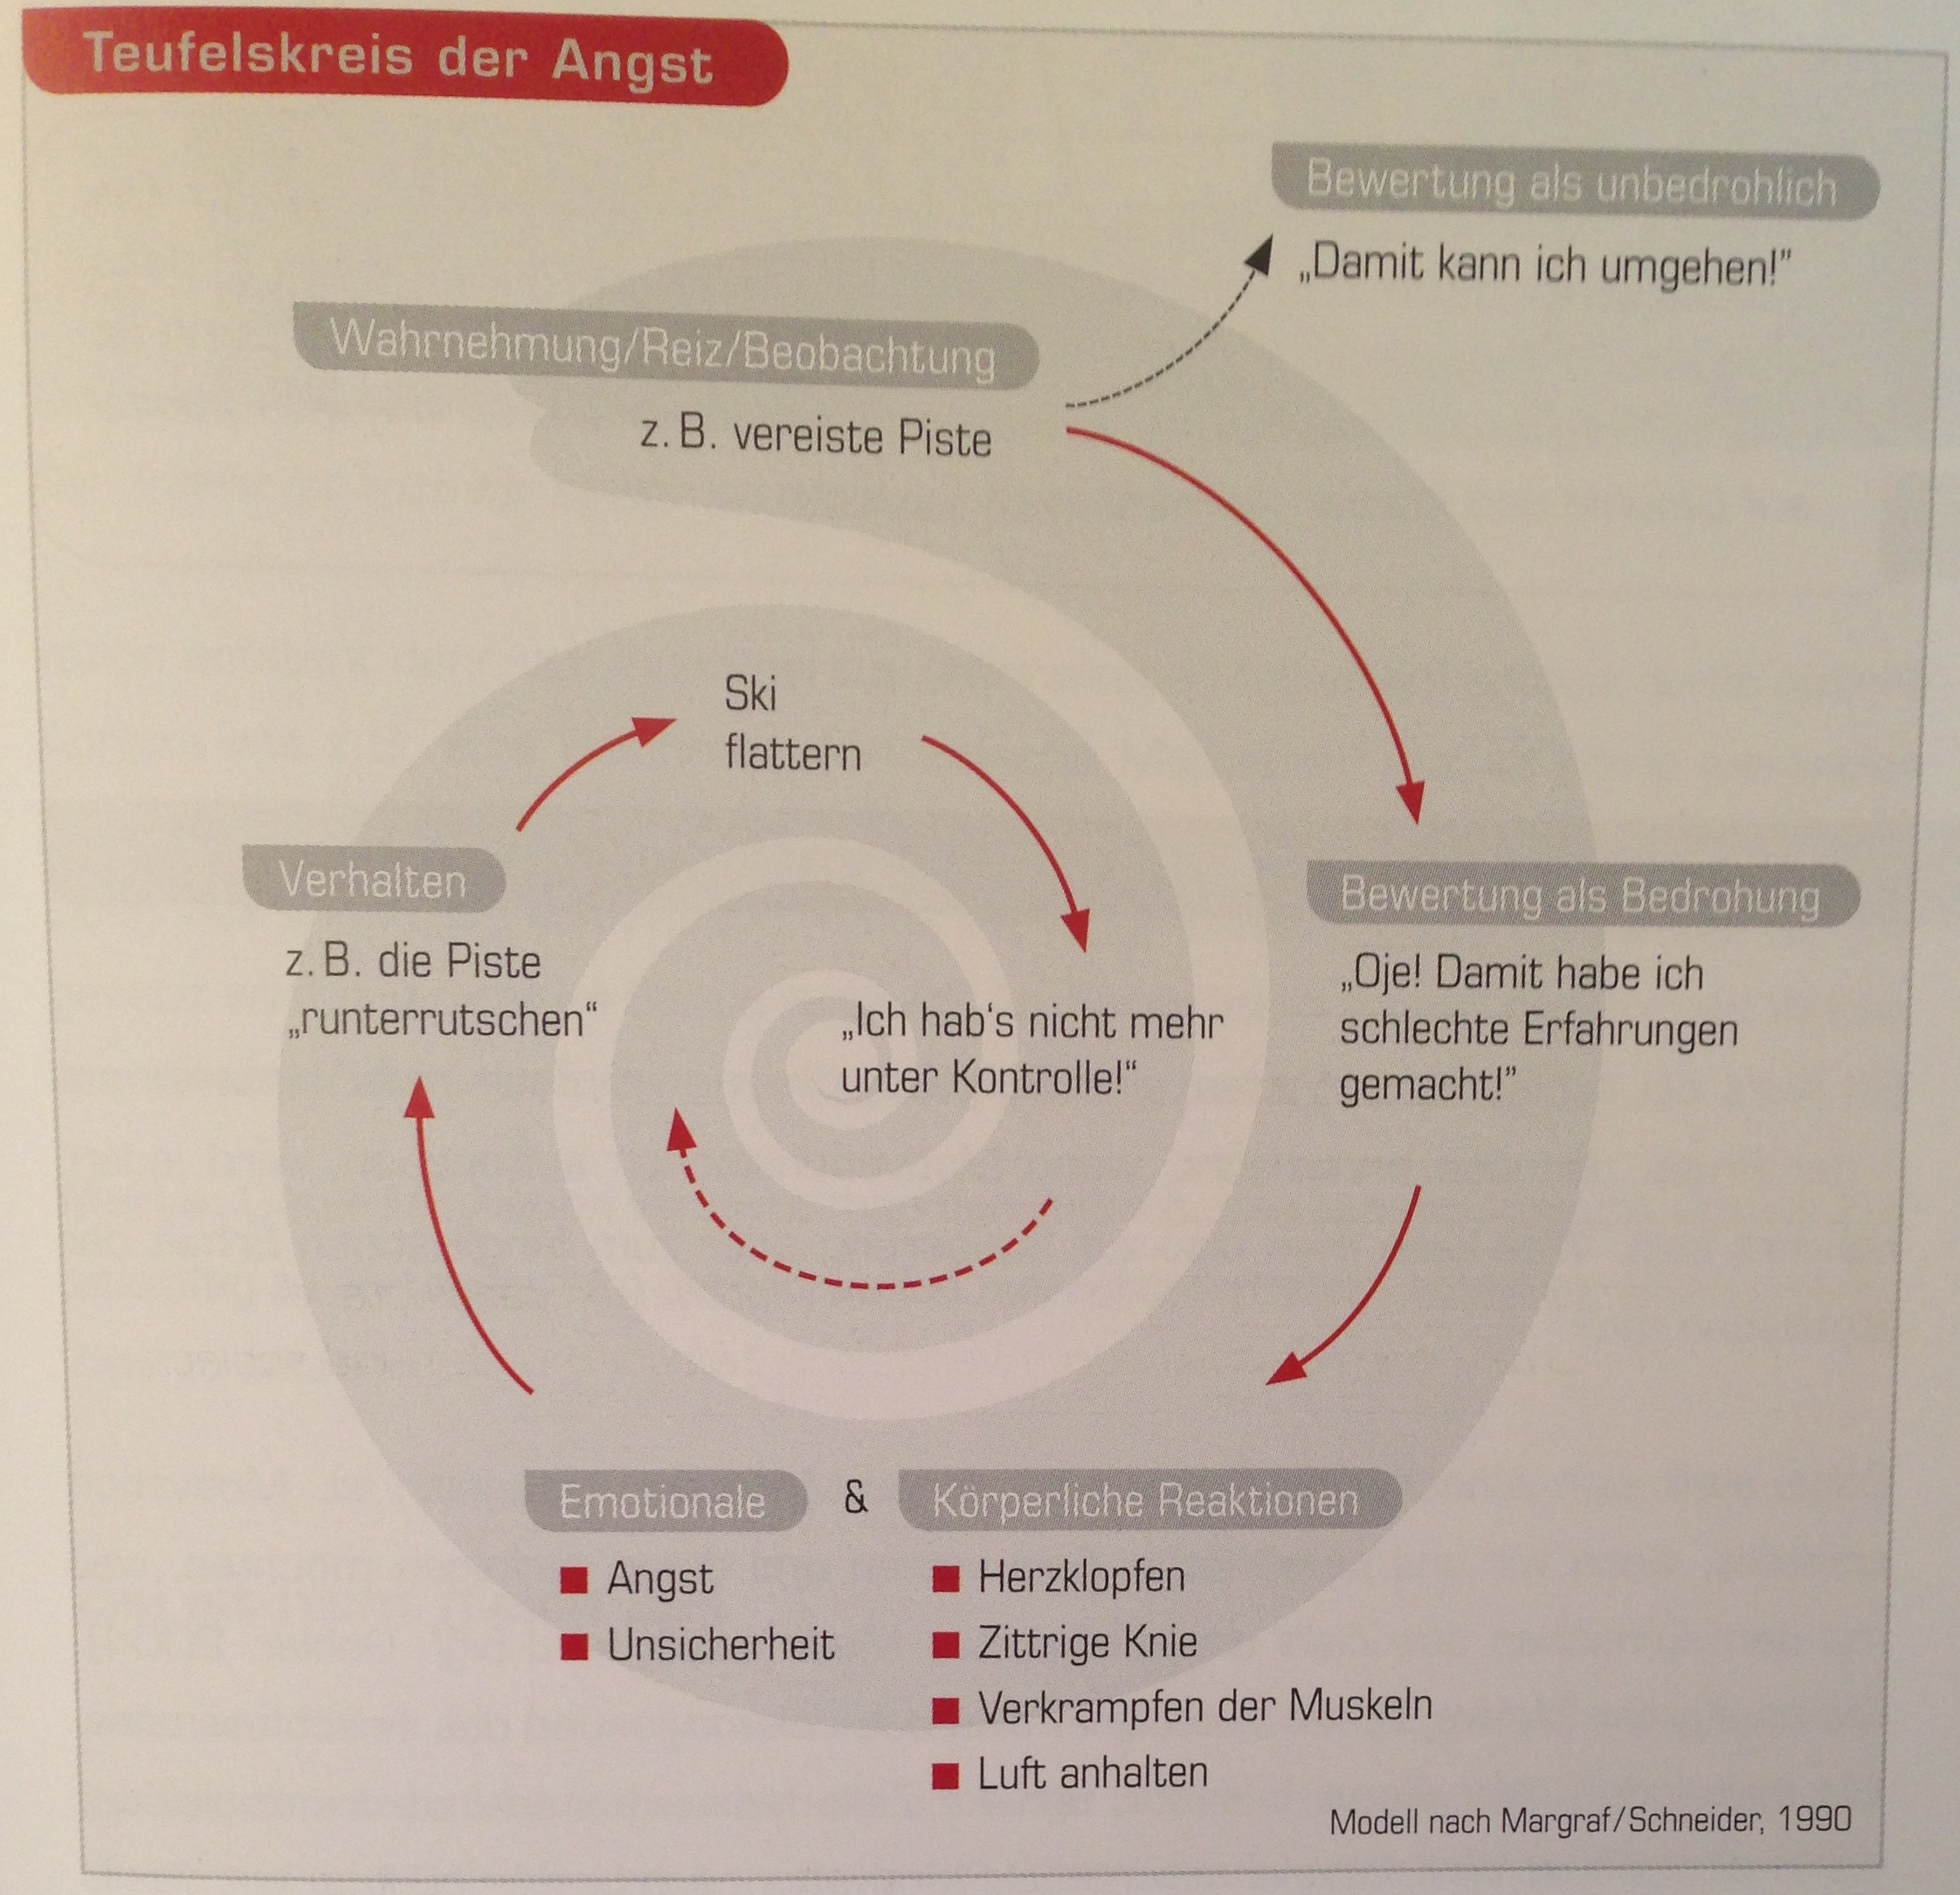
\includegraphics[width=12cm]{pic/angst.jpg}
  \caption{Teufelskreis der Angst.}
  \label{fig:angst}
\end{figure}
Was passiert, wenn jemand keine Selbstwirksamkeitserwartung aufbaut und sich z. B. steile Abfahrten, Tiefschneefahrten oder Wettk"ampfe nicht zutraut? Angst macht sich breit und das bereits Gelernte ist viel schlechter abrufbar. Der Sch"uler wird die Aufgabe nicht so gut meistern, wie er es aufgrund seiner technischen Fertigkeiten k"onnte. Am Teufelskreis der Angst von Margraf und Schneider (1990) wird deutlich, wie sehr Gef"uhle. Gedanken und Verhalten zusammenh"angen und sich aufschaukeln k"onnen und wo man eingreifen kann, um der lch-kann-nicht-Falle zu entkommen.\\\\
\citetitle{theorie} Seite 267
\end{solution}

\begin{question}{2}
Nennen Sie vier Entspannungsverfahren, die in der Sportpsychologie angewendet werden.
\end{question}
\begin{solution}
\begin{itemize}
\item Autogenes Training
\item Progressive Muskelentspannung
\item Atemtechniken
\item Meditation
\end{itemize}
Quelle nicht gefunden.
\end{solution}
%\section{Biomechanik}

\begin{question}{6}
    Definieren Sie den Begriff der Biomechanik. Gehen Sie in diesem Zusammenhang auf relevante Kräfte ein.
\end{question}
\begin{solution}
    Frage noch nicht bearbeitet. Bitte melde dich in einer Mail (Mailadresse auf dem Titelblatt) oder nutze git, wenn du eine Lösung für die Frage hast. Alle anderen können dann von einer korrekten Lösung profitieren.
\end{solution}

\begin{question}{3}
    Erläutern Sie den Drehimpuls anhand eines selbstgewählten Beispiels.
\end{question}
\begin{solution}
    Frage noch nicht bearbeitet. Bitte melde dich in einer Mail (Mailadresse auf dem Titelblatt) oder nutze git, wenn du eine Lösung für die Frage hast. Alle anderen können dann von einer korrekten Lösung profitieren.
\end{solution}

\begin{question}{3}
    Nennen Sie Kräfte bei einer Geradeausfahrt in der Falllinie. Wie können Sie diese kontrollieren?
\end{question}
\begin{solution}
    Frage noch nicht bearbeitet. Bitte melde dich in einer Mail (Mailadresse auf dem Titelblatt) oder nutze git, wenn du eine Lösung für die Frage hast. Alle anderen können dann von einer korrekten Lösung profitieren.
\end{solution}

\begin{question}{3}
    Was ist die Zentrifugalkraft? Beschreiben Sie das dynamische Gleichgewicht.
\end{question}
\begin{solution}
    Frage noch nicht bearbeitet. Bitte melde dich in einer Mail (Mailadresse auf dem Titelblatt) oder nutze git, wenn du eine Lösung für die Frage hast. Alle anderen können dann von einer korrekten Lösung profitieren.
\end{solution}

\begin{question}{3}
    Nennen und erläutern Sie drei Möglichkeiten zur Verringerung des Kurvenradius.
\end{question}
\begin{solution}
    Frage noch nicht bearbeitet. Bitte melde dich in einer Mail (Mailadresse auf dem Titelblatt) oder nutze git, wenn du eine Lösung für die Frage hast. Alle anderen können dann von einer korrekten Lösung profitieren.
\end{solution}

\begin{question}{4}
    Was ist (physikalischer) Druck? Wie kann der Druck im Kurvenverlauf verändert werden? Wozu ist Druck im Kurvenverlauf notwendig?
\end{question}
\begin{solution}
    Frage noch nicht bearbeitet. Bitte melde dich in einer Mail (Mailadresse auf dem Titelblatt) oder nutze git, wenn du eine Lösung für die Frage hast. Alle anderen können dann von einer korrekten Lösung profitieren.
\end{solution}

\begin{question}{5}
    Nennen Sie die Möglichkeiten, den Radius ihres Schneesportgeräts zu verändern. Beschreiben Sie eine Möglichkeit davon detailliert.
\end{question}
\begin{solution}
    Frage noch nicht bearbeitet. Bitte melde dich in einer Mail (Mailadresse auf dem Titelblatt) oder nutze git, wenn du eine Lösung für die Frage hast. Alle anderen können dann von einer korrekten Lösung profitieren.
\end{solution}

\begin{question}{2}
    Wie lässt sich die Taillierung des Schneesportgeräts durch eine Vor- und Rückbewegung verändern?
\end{question}
\begin{solution}
    Frage noch nicht bearbeitet. Bitte melde dich in einer Mail (Mailadresse auf dem Titelblatt) oder nutze git, wenn du eine Lösung für die Frage hast. Alle anderen können dann von einer korrekten Lösung profitieren.
\end{solution}

\begin{question}{2}
    Beschreiben Sie den Verlauf der Druckregulation bei einer Tiefbewegung und einer Hochbewegung.
\end{question}
\begin{solution}
    Frage noch nicht bearbeitet. Bitte melde dich in einer Mail (Mailadresse auf dem Titelblatt) oder nutze git, wenn du eine Lösung für die Frage hast. Alle anderen können dann von einer korrekten Lösung profitieren.
\end{solution}
%\section{Bewegungslehre}

\begin{question}{5}
    Nennen Sie die fünf Sinnesorgane der Sensorik und erläutern Sie diese jeweils anhand eines Beispiels.
\end{question}
\begin{solution}
    Frage noch nicht bearbeitet. Bitte melde dich in einer Mail (Mailadresse auf dem Titelblatt) oder nutze git, wenn du eine Lösung für die Frage hast. Alle anderen können dann von einer korrekten Lösung profitieren.
\end{solution}

\begin{question}{6}
    Beschreiben Sie das kybernetische Regelkreismodell. Welche Schlussfolgerungen ziehen Sie daraus für Ihren Unterricht?
\end{question}
\begin{solution}
    Frage noch nicht bearbeitet. Bitte melde dich in einer Mail (Mailadresse auf dem Titelblatt) oder nutze git, wenn du eine Lösung für die Frage hast. Alle anderen können dann von einer korrekten Lösung profitieren.
\end{solution}

\begin{question}{6}
    Beschreiben Sie einen modernen theoretischen Ansatz des Bewegungslernens.
\end{question}
\begin{solution}
    Frage noch nicht bearbeitet. Bitte melde dich in einer Mail (Mailadresse auf dem Titelblatt) oder nutze git, wenn du eine Lösung für die Frage hast. Alle anderen können dann von einer korrekten Lösung profitieren.
\end{solution}

\begin{question}{6}
    Stellen Sie traditionelle und moderne Lehr- und Lernkonzepte gegenüber. Gehen Sie dabei auf Vor- und Nachteile ein.
\end{question}
\begin{solution}
    Frage noch nicht bearbeitet. Bitte melde dich in einer Mail (Mailadresse auf dem Titelblatt) oder nutze git, wenn du eine Lösung für die Frage hast. Alle anderen können dann von einer korrekten Lösung profitieren.
\end{solution}

\begin{question}{4}
    Kategorisieren Sie die Sportarten nach Aufgabentypen. Geben Sie jeweils ein Beispiel.
\end{question}
\begin{solution}
    Frage noch nicht bearbeitet. Bitte melde dich in einer Mail (Mailadresse auf dem Titelblatt) oder nutze git, wenn du eine Lösung für die Frage hast. Alle anderen können dann von einer korrekten Lösung profitieren.
\end{solution}

\begin{question}{5}
    Beschreiben Sie das Modell des differenziellen Lernens.
\end{question}
\begin{solution}
    Frage noch nicht bearbeitet. Bitte melde dich in einer Mail (Mailadresse auf dem Titelblatt) oder nutze git, wenn du eine Lösung für die Frage hast. Alle anderen können dann von einer korrekten Lösung profitieren.
\end{solution}

\begin{question}{2}
    Definieren Sie den Begriff Techniktraining.
\end{question}
\begin{solution}
    Frage noch nicht bearbeitet. Bitte melde dich in einer Mail (Mailadresse auf dem Titelblatt) oder nutze git, wenn du eine Lösung für die Frage hast. Alle anderen können dann von einer korrekten Lösung profitieren.
\end{solution}

\begin{question}{4}
    Beschreiben Sie den Unterschied zwischen Ziel- und Handlungsorientierung.
\end{question}
\begin{solution}
    Frage noch nicht bearbeitet. Bitte melde dich in einer Mail (Mailadresse auf dem Titelblatt) oder nutze git, wenn du eine Lösung für die Frage hast. Alle anderen können dann von einer korrekten Lösung profitieren.
\end{solution}

\begin{question}{6}
    Nennen Sie vier Grundsätze der Methodik im Techniktraining aus Sicht des DSV und erläutern Sie diese.
\end{question}
\begin{solution}
    Frage noch nicht bearbeitet. Bitte melde dich in einer Mail (Mailadresse auf dem Titelblatt) oder nutze git, wenn du eine Lösung für die Frage hast. Alle anderen können dann von einer korrekten Lösung profitieren.
\end{solution}

\begin{question}{6}
    Worauf müssen Sie bei der Rückmeldung an Ihren Schüler achten? Geben Sie drei Beispiele und erläutern Sie diese.
\end{question}
\begin{solution}
    Frage noch nicht bearbeitet. Bitte melde dich in einer Mail (Mailadresse auf dem Titelblatt) oder nutze git, wenn du eine Lösung für die Frage hast. Alle anderen können dann von einer korrekten Lösung profitieren.
\end{solution}
%\section{Trainingslehre}

\begin{question}{3}
    Skizzieren Sie das theoretische Modell der Superkompensation.
\end{question}
\begin{solution}
    Frage noch nicht bearbeitet. Bitte melde dich in einer Mail (Mailadresse auf dem Titelblatt) oder nutze git, wenn du eine Lösung für die Frage hast. Alle anderen können dann von einer korrekten Lösung profitieren.
\end{solution}

\begin{question}{4}
    Nennen und beschreiben Sie die vier konditionellen Fähigkeiten und deren Bedeutung für Ihre Disziplin.
\end{question}
\begin{solution}
    Frage noch nicht bearbeitet. Bitte melde dich in einer Mail (Mailadresse auf dem Titelblatt) oder nutze git, wenn du eine Lösung für die Frage hast. Alle anderen können dann von einer korrekten Lösung profitieren.
\end{solution}

\begin{question}{5}
    Nennen Sie die leistungsbestimmenden Faktoren auf die sportliche Leistung allgemein. Geben Sie zu jedem Faktor ein Beispiel aus dem Schneesport an, das seinen Einflussbeschreibt.
\end{question}
\begin{solution}
    Frage noch nicht bearbeitet. Bitte melde dich in einer Mail (Mailadresse auf dem Titelblatt) oder nutze git, wenn du eine Lösung für die Frage hast. Alle anderen können dann von einer korrekten Lösung profitieren.
\end{solution}

\begin{question}{6}
    Definieren Sie den Begriff der Ausdauer. Nennen und beschreiben Sie kurz drei Trainingsmethoden zur Verbesserung der Ausdauerleistungsfähigkeit.
\end{question}
\begin{solution}
    Frage noch nicht bearbeitet. Bitte melde dich in einer Mail (Mailadresse auf dem Titelblatt) oder nutze git, wenn du eine Lösung für die Frage hast. Alle anderen können dann von einer korrekten Lösung profitieren.
\end{solution}

\begin{question}{4}
    Welche Faktoren beeinflussen die motorische Kraft?
\end{question}
\begin{solution}
    Frage noch nicht bearbeitet. Bitte melde dich in einer Mail (Mailadresse auf dem Titelblatt) oder nutze git, wenn du eine Lösung für die Frage hast. Alle anderen können dann von einer korrekten Lösung profitieren.
\end{solution}

\begin{question}{6}
    Definieren Sie den Begriff der motorischen Kraft. Nennen und beschreiben Sie kurz vier motorische Kraftfähigkeiten.
\end{question}
\begin{solution}
    Frage noch nicht bearbeitet. Bitte melde dich in einer Mail (Mailadresse auf dem Titelblatt) oder nutze git, wenn du eine Lösung für die Frage hast. Alle anderen können dann von einer korrekten Lösung profitieren.
\end{solution}

\begin{question}{6}
    Beschreiben Sie, welche Komponenten die Maximalkraft beeinflussen und beschreiben Sie zwei Trainingsmethoden zum Training der Maximalkraft.
\end{question}
\begin{solution}
    Frage noch nicht bearbeitet. Bitte melde dich in einer Mail (Mailadresse auf dem Titelblatt) oder nutze git, wenn du eine Lösung für die Frage hast. Alle anderen können dann von einer korrekten Lösung profitieren.
\end{solution}

\begin{question}{2}
    Definieren Sie den Begriff Training.
\end{question}
\begin{solution}
    Frage noch nicht bearbeitet. Bitte melde dich in einer Mail (Mailadresse auf dem Titelblatt) oder nutze git, wenn du eine Lösung für die Frage hast. Alle anderen können dann von einer korrekten Lösung profitieren.
\end{solution}

\begin{question}{7}
    Nennen und beschreiben Sie die koordinativen Fähigkeiten nach Weineck (2010).
\end{question}
\begin{solution}
    Frage noch nicht bearbeitet. Bitte melde dich in einer Mail (Mailadresse auf dem Titelblatt) oder nutze git, wenn du eine Lösung für die Frage hast. Alle anderen können dann von einer korrekten Lösung profitieren.
\end{solution}

\begin{question}{4}
    Beschreiben Sie die Besonderheiten im Kinder- und Jugendtraining für den Bereich \emph{Ausdauer/Kraft/Koordination}.
\end{question}
\begin{solution}
    Frage noch nicht bearbeitet. Bitte melde dich in einer Mail (Mailadresse auf dem Titelblatt) oder nutze git, wenn du eine Lösung für die Frage hast. Alle anderen können dann von einer korrekten Lösung profitieren.
\end{solution}
%\section{Ernährung}

\begin{question}{6}
    Worauf ist bei einer gesunden und ausgewogenen Ernährung zu achten?
\end{question}
\begin{solution}
    Frage noch nicht bearbeitet. Bitte melde dich in einer Mail (Mailadresse auf dem Titelblatt) oder nutze git, wenn du eine Lösung für die Frage hast. Alle anderen können dann von einer korrekten Lösung profitieren.
\end{solution}

\begin{question}{6}
    Geben Sie Tipps für die Ernährung während eines Unterrichtstages auf Schnee für Ihre Disziplin.
\end{question}
\begin{solution}
    Frage noch nicht bearbeitet. Bitte melde dich in einer Mail (Mailadresse auf dem Titelblatt) oder nutze git, wenn du eine Lösung für die Frage hast. Alle anderen können dann von einer korrekten Lösung profitieren.
\end{solution}

\printbibliography

\end{document}